\documentclass[sigplan,screen]{acmart}
\settopmatter{printfolios=true,printccs=true,printacmref=true}
\copyrightyear{2020}
\acmYear{2020}
\setcopyright{acmlicensed}
%\acmConference[LICS '20]{Proceedings of the 35th Annual ACM/IEEE Symposium on Logic in Computer Science}{July 8--11, 2020}{Saarbrücken, Germany}
\acmConference[LICS '20]{Proceedings of the 35th Annual ACM/IEEE Symposium on Logic in Computer Science (LICS)}{July 8--11, 2020}{Saarbr\"ucken, Germany}
\acmBooktitle{Proceedings of the 35th Annual ACM/IEEE Symposium on Logic
in Computer Science (LICS '20), July 8--11, 2020, Saarbr\"ucken, Germany}
\acmPrice{15.00}
\acmDOI{10.1145/3373718.3394799}
\acmISBN{978-1-4503-7104-9/20/07}

\usepackage{amsmath} % in acmart, but helps vim syntax highlighting
\usepackage{tikz-cd}
\usepackage{bbm}
\usepackage{ebproof}
\usepackage{stmaryrd}
\usepackage{color,soul}

% Macros {{{

\newcommand{\gcat}{\mathcal{G}_{\sqsubseteq}}
\newcommand{\kw}[1]{\ensuremath{ \mathsf{#1} }}
\newcommand{\ifr}[1]{\mathrel{[{#1}]}}
\newcommand{\bdot}{\boldsymbol{\cdot}}
\newcommand{\plays}[4]{{ {#1}_{{#2} \rightarrow {#3}}[{#4}] }}
\newcommand{\pplays}[3]{\plays{\bar{P}}{#1}{#2}{#3}}
\newcommand{\oplays}[3]{\plays{P}{#1}{#2}{#3}}
\newcommand{\htr}[3]{{ {#1} \mathbbm{\{} {#2} \mathbbm{\}} {#3} }}
\newcommand{\ignore}[1]{}

\newcommand{\hlc}[2][yellow]{ {\sethlcolor{#1} \hl{#2}} }
\newcommand\zhong[1]{\hlc[yellow]{[Zhong: #1]}}
\newcommand\jk[1]{\hlc[pink]{[Jeremie: #1]}}

\hyphenation{Comp-Cert}
\hyphenation{Comp-CertX}
\newcommand{\sbt}{\,\begin{picture}(-1,1)(-1,-3)\circle*{3}\end{picture}\ }
%}}}

\begin{document}

\pagestyle{empty}


\title{Refinement-Based Game Semantics for Certified Abstraction Layers} %{{{

\author{J\'er\'emie Koenig}
\affiliation{Yale University}
\email{jeremie.koenig@yale.edu}

\author{Zhong Shao}
\affiliation{Yale University}
\email{zhong.shao@yale.edu}

%}}}

\begin{abstract} %{{{
Formal methods have advanced to the point where
the functional correctness of various large
system components has been mechanically verified.
However,
the variety of semantic models used across projects
makes it difficult to connect these component
to build larger certified systems.
%Therefore,
Given this,
we seek to embed these models and proofs
into a general-purpose framework
where they could interact. %be made interoperable.
%linked together to
%construct certified heterogeneous systems.
We believe that a synthesis of game
semantics, the refinement calculus, and algebraic effects can
provide such a framework.

To combine game semantics and refinement, we replace the downset
completion typically used to construct strategies from posets of plays.
Using the \emph{free completely distributive completion},
we construct \emph{strategy specifications}
equipped with arbitrary angelic and demonic choices
and ordered by a generalization of alternating refinement.
This provides a novel approach to nondeterminism in game semantics.

%To connect
Connecting algebraic effects and game semantics, we interpret effect
signatures as games and define two
categories %$\gcat^{ib}$ and $\gcat^b$
of effect signatures and strategy
specifications.
The resulting models are sufficient to represent the behaviors
of a variety of low-level components,
including the \emph{certified abstraction layers}
used to verify the operating system
kernel CertiKOS. %~\cite{popl15}.
\end{abstract}
%}}}

%% keywords {{{
%% 2012 ACM Computing Classification System (CSS) concepts
%% Generate at 'http://dl.acm.org/ccs/ccs.cfm'.
\begin{CCSXML}
<ccs2012>
<concept>
<concept_id>10003752.10010124.10010138.10010140</concept_id>
<concept_desc>Theory of computation~Program specifications</concept_desc>
<concept_significance>500</concept_significance>
</concept>
<concept>
<concept_id>10003752.10010124.10010138.10010142</concept_id>
<concept_desc>Theory of computation~Program verification</concept_desc>
<concept_significance>500</concept_significance>
</concept>
<concept>
<concept_id>10003752.10010124.10010138.10011119</concept_id>
<concept_desc>Theory of computation~Abstraction</concept_desc>
<concept_significance>500</concept_significance>
</concept>
<concept>
<concept_id>10011007.10011006.10011039.10011311</concept_id>
<concept_desc>Software and its engineering~Semantics</concept_desc>
<concept_significance>500</concept_significance>
</concept>
<concept>
<concept_id>10011007.10010940.10010992.10010993.10010994</concept_id>
<concept_desc>Software and its engineering~Functionality</concept_desc>
<concept_significance>500</concept_significance>
</concept>
</ccs2012>
\end{CCSXML}

\ccsdesc[500]{Theory of computation~Program specifications}
\ccsdesc[500]{Theory of computation~Program verification}
\ccsdesc[500]{Theory of computation~Abstraction}
\ccsdesc[500]{Software and its engineering~Semantics}
\ccsdesc[500]{Software and its engineering~Functionality}
%% End of generated code

%% Keywords
%% comma separated list
\keywords{certified abstraction layers; dual nondeterminism; game semantics; strategy specification; program refinement; interaction specification; algebraic effects}
%% \keywords are mandatory in final camera-ready submission
%}}}

\maketitle
\thispagestyle{empty}
\section{Introduction} \label{sec:intro} %{{{

% Preamble: certified software {{{

Certified software~\cite{shao10}
is software accompanied by
mechanized, machine-checkable proofs of correctness.
To construct a certified program,
we must not only write its code in a given programming language,
but also formally specify its intended behavior
and construct, using specialized tools,
evidence that the program
indeed conforms to the specification.

%To achieve this,
%we need formal models of
%the languages in which they are described.
%The tools used to reason about them
%should be sound with respect to these models.
%Ideally,
%this will be demonstrated in an established,
%%general-purpose proof assistant,
%diminishing the possibility that
%incorrect programs will be validated because of
%accidental or deliberate mistake
%in the software used to construct and check proofs.

%}}}

\subsection{Certified systems at scale} %{{{
\label{ssec:certsys}

The past decade has seen an explosion
in the scope and scale of practical software verification.
Researchers have been able to produce certified
compilers \cite{compcert},
program logics \cite{vst},
operating system kernels \cite{sel4,popl15},
file systems \cite{fscq} and more,
often introducing new techniques
and mathematical models.
In this context,
there has been increasing interest in
making these components
interoperable and
combining them---and their proofs of correctness---%
into larger certified systems.

This is exemplified by the DeepSpec project \cite{deepspec},
which seeks to connect various components
specified and verified in the Coq proof assistant.
The key idea behind DeepSpec
is to interpret specifications as \emph{interfaces}
between components.
When a component providing a certain interface
has been verified,
client components can rely on this
for their own proofs of correctness.
Standardizing this process would make it possible
to construct large-scale certified systems
by assembling off-the-shelf certified components.

%This approach would provides benefits
%beyond the potential increase in the scale of
%practical certified system.
%As it stands,
%a certified system is only
%as trustworthy as its specification.
%Indeed,
%it is possible to prove a buggy system correct
%with respect to a buggy specification.
%If the only user of the specification
%is a human expert subjecting it to careful examination,
%these bugs could go unnoticed
%and persist in the final system.
%By contrast,
%if we attempt to use the same specification as a dependency
%in the correctness proof of a client component,
%its deficiencies will become apparent
%and prevent us from carrying out this second proof of correctness.
%Moreover,
%the internal specifications used
%as intermediate steps
%in the verification of a complex system
%disappear from the external characterization of the system,
%and no longer need to be trusted.
%This reduces the ratio between the size of the system
%and the size of the specification
%which must be trusted and understood
%to establish guarantees about the overall system.

To an extent,
these principles are already demonstrated in the structure of the
certified C compiler CompCert \cite{compcert},
where the semantics of intermediate languages
serve as intermediate specifications for each compilation pass.
The correctness of each pass is established by
proving that the behavior of its target program
refines that of its source program.
%(which serves in this case as the specification).
As passes are composed to obtain the overall
C-to-assembly compiler,
the correctness proofs are composed as well
to construct a correctness proof for the whole compiler.
The final theorem does not mention the intermediate
programs and language semantics,
so that a user only needs to trust
the accuracy of CompCert's C and assembly semantics,
and the soundness of the proof assistant.

Building on this precedent,
the CertiKOS verification effort~\cite{popl15,ccal,osdi16}
divided the kernel into several dozen abstraction layers
which were then specified and verified individually.
Layer specifications provide
an abstract view of a layer's functionality,
hiding the procedural details and low-level data representations
involved in its implementation.
Client code can be verified in terms of
this abstract view
in order to build higher-level layers.
Certified layers
with compatible interfaces can then be chained together
in the way passes of a compiler
can be composed when the target language of one
corresponds to the source language of the other.

%}}}

\subsection{Semantic models for verification} %{{{
\label{ssec:semant}

While this approach is compelling,
there are difficulties associated with extending it
to build larger-scale certified systems
by connecting disparate certified components.
A key aspect enabling composition in CompCert and CertiKOS
is the uniformity of the models underlying
their language semantics and correctness proofs.
By contrast,
across projects
there exist a great diversity
of semantic models and verification techniques.
This makes it difficult to formulate
interface specifications to connect specific components,
let alone devising a general system
to express such interfaces.

Worse yet,
this diversity is not simply a historical accident.
The semantic models
used in the context of individual verification projects
are often carefully chosen
to make the verification task tractable.
The semantic model used in CompCert alone
has changed multiple times,
addressing new requirements and techniques
that were introduced alongside
new compiler features and optimizations~\cite{compsem}.
Given the difficulty of verification,
preserving this flexibility is essential.

Then,
to make it possible to link components
verified using a variety of paradigms,
we need to identify a model
expressive enough to embed
the semantics, specifications and correctness proofs
of a variety of paradigms.
To enable constructing large-scale certified systems,
the model should provide
high-level composition and reasoning principles.

%}}}

\subsection{General models for system behaviors} %{{{
\label{ssec:genmodel}

Fortunately,
there is a wealth of semantics research to draw from
when attempting to design models for this task.

The framework of
symmetric monoidal categories,
which allows components to be
connected in series~($\circ$) and in parallel~($\otimes$),
captures structures found
in various kinds of systems and processes \cite{rosetta},
and appears in different forms
in many approaches to logic and programming language semantics.

A particularly expressive instance of this phenomenon
is realized in \emph{game semantics} \cite{cspgs},
an approach to compositional semantics
which uses two-player games to model
the interaction between a component and its environment,
and represents the externally observable behavior
of the component as a strategy in this game.
The generality of games as
descriptions of the possible interactions of components
makes this approach broadly applicable,
and the typed aspect of the resulting models
makes it ideal to the task of
describing the behavior of heterogeneous systems.

However,
the generality of game models
often translates to a fair amount of complexity,
which imposes a high barrier to entry for practitioners
and makes them difficult to formalize in a proof assistant.
While more restricted,
the framework of \emph{algebraic effects} \cite{effadq}
is sufficient for many modeling tasks,
fits within the well-known monadic approach
to effectful and interactive computations,
and can be adapted into a particularly simple version
of game semantics.
Along these lines,
\emph{interaction trees} \cite{itree}
have been developed for use in and across
several DeepSpec projects.

%\subsection{General formulations for correctness proofs}
%\label{ssec:genform}

Finally,
while game models have been proposed
for a wide variety of programming languages,
there has been comparatively less focus
on specifications and correctness properties.
%in the context of game semantics.
By contrast,
the general approach of \emph{stepwise refinement}
suggests a uniform treatment of programs, specifications
and their relationships.
It has been studied extensively in the context of
%Dijkstra's
predicate transformer semantics \cite{gc}
and in the framework known as the \emph{refinement calculus} \cite{refcal}.

%In refinement-based approaches,
%programs and specifications are expressed in a common language,
%and a certified program is constructed in an incremental manner,
%by applying a series of correctness-preserving transformation
%to the (abstract and declarative) specification
%until we obtain a (concrete and executable) program.
%Correctness preservation is expressed
%by a reflexive and transitive \emph{refinement relation} $\sqsubseteq$.
%Language constructions are monotonic with respect to $\sqsubseteq$,
%so that elementary refinement rules
%can be applied congruently within any program context.
%
%To make it possible to express specifications,
%the language is extended with non-executable constructions,
%including in particular infinitary versions of both
%\emph{angelic} and \emph{demonic} nondeterministic choice operators.
%In its modern presentation,
%the refinement calculus is formulated in a lattice-theoretic framework
%where joins ($\sqcup$) and meets ($\sqcap$)
%correspond respectively to angelic and demonic choices.
%The resulting language is remarkably expressive
%and requires very few additional primitive constructions.
%The duality inherent in this approach
%also lends itself to game-theoretic interpretations,
%and indeed the semantics of the refinement calculus
%can be expressed as a two-player game between
%the angel and the demon \cite{refcal}.
%
%Like all approaches in the lineage of Hoare logic
%and predicate transformer semantics,
%the refinement calculus is limited to
%modelling imperative programs.
%[However,
%M\&T propose to extend it to terms and functional programming
%by constructing the FCD blah blah.]
%
%[Also: describe the idea of the \emph{refinement calculus hierarchy}
%(general and difficult <-> specific and easy to reason about
%and string properties).
%More than one level of ``semantics''
%Notions of ``syntax'' and ``semantics'' are relative concepts.]
%
%}}}

%\zhong{Maybe we should shorten the last two subsections a bit so we can get to the contributions sooner.}

\subsection{Contributions} %{{{
\label{ssec:contrib}

Our central claim is that a synthesis
of %the existing research on
game semantics, algebraic effects, and the refinement calculus
can be used to construct a hierarchy of semantic models
suitable for constructing large-scale, heterogeneous certified systems.
To provide evidence for this claim,
we outline general techniques
which can realize this synthesis
and demonstrate their use
in the context of certified abstraction layers:
\begin{itemize}
\item
  We adapt the work of Morris and Tyrrell \cite{augtyp,dndf},
  which extends the refinement calculus to the level of terms
  by using \emph{free completely distributive completions} of posets,
  to investigate \emph{dual nondeterminism}
  in the context of game semantics
  %Using the free completely distributive completion
  %instead of downsets when constructing strategies
  %yields
  and construct
  completely distributive lattices of
  \emph{strategy specifications},
  partially ordered
  under a form of alternating refinement
  \cite{altref}.
\item
  In \S\ref{sec:intspec},
  we define a version of the
  \emph{free monad on an effect signature}
  which incorporates dual nondeterminism and refinement.
  The result can be used to formulate a theory of certified abstraction
  layers in which
  layer interfaces, layer implementations, and abstraction relations
  are treated uniformly and compositionally.
\item
  In \S\ref{sec:gamesem},
  we outline a more general category of games and
  strategy specifications;
  its object are effect signatures regarded as games
  and its morphisms specify well-bracketed strategies.
  The behavior of certified abstraction layers
  can then be represented canonically,
  and reentrant layer interfaces can be modeled.
\end{itemize}

The model presented in \S\ref{sec:intspec} was designed to be simple but
general enough to embed CompCert semantics, certified
abstraction layers, and interaction trees. The main purpose for
the model presented in \S\ref{sec:gamesem} is then to hide state and
characterize certified abstraction layers through
their externally observable interactions only.

Note that rather than providing
denotational semantics for specific programming
languages, our models are intended as a coarse-grained composition
``glue'' between components developed and verified in their own
languages, each equipped with their own internal semantics.
In this context,
the models' restriction to first-order computation
applies only to cross-component interactions,
and conforms to our interest in connecting
%relatively
low-level system components.

%They could be embedded in turn
%into more general game models, for instance where concurrency
%could be expressed in a more natural way.

%}}}

%}}}

\section{Background and approach} \label{sec:background} %{{{

% Preamble {{{

The work presented in this paper
draws from a broad range of existing research.
This section summarizes the relevant aspects
of these various lines of work,
and outlines how we combine them
to develop
refinement-based game semantics.

%}}}

\subsection{Dual nondeterminism and refinement} \label{sec:refcal} %{{{

% Preamble {{{

Correctness properties for imperative programs
are often stated as triples of the form $\htr{P}{C}{Q}$
asserting that
when the program $C$ is started in a state which
satisfies the predicate $P$ (the \emph{precondition}),
then the state in which $C$ terminates
will satisfy the predicate $Q$ (the \emph{postcondition}).
For example:
\[
    \htr{\text{$\kw{x}$ is odd}\,}{\kw{x := x * 2}}{\,\text{$\kw{x}$ is even}}
\]
In the \emph{axiomatic} approach~\cite{hoare69} to programming language semantics,
inference rules
corresponding to the different constructions of the language
determine which triples are valid,
and the meaning of a program is identified with
the set of properties $\htr{P}{-}{Q}$
which the program satisfies.

Axiomatic semantics
can accommodate nondeterminism in two different ways.
In the program $C_1 \sqcap C_2$,
a \emph{demon} will choose which of $C_1$ or $C_2$ is executed.
The program $\kw{x := 2 * x} \: \sqcap \: \kw{x := 0}$
may be executed arbitrarily as $\kw{x := 2 * x}$ or $\kw{x := 0}$,
with no guarantee as to which branch will be chosen.
The demon works against us,
so that if we want $C_1 \sqcap C_2$ to satisfy a given property,
we need to make sure we can deal with either choice.
This corresponds to the inference rule:
\[
  \begin{prooftree}
    \hypo{\htr{P}{C_1}{Q}}
    \hypo{\htr{P}{C_2}{Q}}
    \infer2{\htr{P}{C_1 \sqcap C_2}{Q}}
  \end{prooftree}
\]
Conversely,
in the program $C_1 \sqcup C_2$,
an \emph{angel} will decide whether $C_1$ or $C_2$ is executed.
If possible,
the angel will make choices which validate
the correctness property.
This implies:
\[
  \begin{prooftree}
    \hypo{\htr{P}{C_1}{Q}}
    \infer1{\htr{P}{C_1 \sqcup C_2}{Q}}
  \end{prooftree}
  \qquad
  \begin{prooftree}
    \hypo{\htr{P}{C_2}{Q}}
    \infer1{\htr{P}{C_1 \sqcup C_2}{Q}}
  \end{prooftree}
\]
The statement $\kw{x := x * 2} \: \sqcup \: \kw{x := 0}$
is more difficult to interpret than its demonic counterpart,
but can be thought of as a program which magically behaves as
$\kw{x := x * 2}$ or $\kw{x := 0}$
depending on the needs of its user.

More generally,
a triple $\htr{P}{C}{Q}$
can be interpreted as a \emph{game}
between the angel and the demon \cite{refcal}.
The angel resolves the $\sqcup$ choices,
whereas the demon resolves $\sqcap$.
The triple is valid if there is a winning strategy
for the angel.

%}}}

%\paragraph{Distributivity} %{{{
%
%Note that in this setup,
%$\sqcap$ and $\sqcup$ distribute over each other.
%More precisely, for all $P, C_1, C_2, C_3, Q$:
%\begin{align*}
%  \htr{P}{C_1 \sqcap (C_2 \sqcup C_3)}{Q} &\Leftrightarrow
%    \htr{P}{(C_1 \sqcap C_2) \sqcup (C_1 \sqcap C_3)}{Q} \\
%  \htr{P}{C_1 \sqcup (C_2 \sqcap C_3)}{Q} &\Leftrightarrow
%    \htr{P}{(C_1 \sqcup C_2) \sqcap (C_1 \sqcup C_3)}{Q}
%\end{align*}
%Consider the first equivalence above.
%If the angel has a winning strategy for
%the left-hand side triple,
%they can win both $\htr{P}{C_1}{Q}$
%and either $\htr{P}{C_2}{Q}$ or $\htr{P}{C_3}{Q}$.
%Although the right-hand side triple
%reverses the angel and demon's choices,
%the angel can preemptively choose the left or right
%disjunct depending on whether they can win
%$\htr{P}{C_2}{Q}$ or $\htr{P}{C_3}{Q}$.
%Likewise, if the angel can win the right-hand side,
%then they have a winning strategy for the left-hand side as well.
%The second equivalence corresponds to a similar situation
%where the angel and demon have been exchanged.
%
%%}}}

\paragraph{Program refinement} %{{{

Instead of proving program correctness in one go,
\emph{stepwise refinement} techniques use a more incremental approach
centered on the notion of program refinement.
A refinement $C_1 \sqsubseteq C_2$
means that any correctness property satisfied by $C_1$
will also be satisfied by $C_2$:
\[
    C_1 \sqsubseteq C_2 \: := \:
    \forall P Q \cdot
      \htr{P}{C_1}{Q} \Rightarrow
      \htr{P}{C_2}{Q}
\]
We say that $C_2$ refines $C_1$
or that $C_1$ is refined by $C_2$.

Typically,
under such approaches,
the language will be extended with constructions
allowing the user to describe
abstract specifications as well as
concrete programs.
The goal will then be to establish
a sequence of refinements
$C_1 \sqsubseteq \cdots \sqsubseteq C_n$
to show that a program $C_n$ involving
only executable constructions
correctly implements a specification $C_1$,
which may be stated in much more abstract terms.

If the language is sufficiently expressive,
then a correctness property $\htr{P}{-}{Q}$
can itself be encoded \cite{specstm} as
a specification statement $\langle{}P,Q{}\rangle$
such that:
\[
    \htr{P}{C}{Q} \: \Leftrightarrow \:
    \langle{}P,Q{}\rangle \sqsubseteq C \,.
\]
In the context of refinement,
the properties associated with demonic and angelic choice
generalize as:
\begin{align*}
  C \sqsubseteq C_1 \:\wedge\: C \sqsubseteq C_2 &
    \:\Rightarrow\: C \sqsubseteq C_1 \sqcap C_2 \\
  C \sqsubseteq C_1 \:\vee\: C \sqsubseteq C_2 &
    \:\Rightarrow\: C \sqsubseteq C_1 \sqcup C_2
\end{align*}
Given the symmetry between the demon and angel,
it is then natural to interpret demonic and angelic choices
respectively as meets and joins
of the refinement ordering.

Until this point,
we have discussed demonic ($\sqcap$) and angelic ($\sqcup$) choices
as implementation constructs
(appearing to the right of $\sqsubseteq$),
taking the point of view of a client
seeking to use the program to achieve a certain goal.
However,
in this work we use them primarily
as \emph{specification} constructs
(appearing to the left of $\sqsubseteq$),
and are interested in what it means
for a system to implement them.
%
As a specification, $C_1 \sqcap C_2$
allows the system to refine either one of $C_1$ or $C_2$, while
$C_1 \sqcup C_2$ requires it to refine
\emph{both} of them:
\begin{gather*}
  C_1 \sqsubseteq C \: \vee \: C_2 \sqsubseteq C
    \: \Rightarrow \: C_1 \sqcap C_2 \sqsubseteq C \\
  C_1 \sqsubseteq C \: \wedge \: C_2 \sqsubseteq C
    \: \Rightarrow \: C_1 \sqcup C_2 \sqsubseteq C 
\end{gather*}
In other words,
demonic choices
give us more
implementation freedom,
whereas angelic choices make a specification
stronger and more difficult to implement.
%Intuitively,
%the \emph{user} of a specification
%will need to be ready to handle any demonic choice
%made in that specification.
%The specification's implementer
%will have more freedom because they \emph{are} the demon.
%Conversely,
%angelic choice requires the implementation
%to behave appropriately
%no matter which alternative the user decides to rely on.
%Therefore,
Therefore we can think of demonic choices as
choices of the \emph{system}, % we are considering,
and think of angelic choices as
choices of the \emph{environment}.

%}}}

\paragraph{The refinement calculus} %{{{

\jk{cut candidate}
These basic ingredients have been studied systematically
in the \emph{refinement calculus},
dating back to Ralph-Johan Back's 1978 PhD thesis \cite{backthesis}.
In its modern incarnation \cite{refcal},
the refinement calculus
subsumes programs and specifications with \emph{contracts}
featuring unbounded angelic and demonic choices.
%These choice operators
%constitute a completely distributive lattice
%with respect to the refinement order.

%Dijkstra's \emph{predicate transformer} semantics \cite{gc}
%are a natural fit for the refinement calculus,
%but other approaches are possible.
%For instance,
%the understanding of contracts as a game between
%the angel and the demon
%can be formalized to provide a form of
%game semantics for the refinement calculus.

%More generally,
The refinement calculus can be presented as a \emph{hierarchy}
where simpler models (state transformer functions, relations)
can be embedded in more general ones (predicate transformers)
in various structure-preserving ways.
This makes it possible to reason about simpler components
in a limited, stronger version of the framework,
while retaining the possibility of embedding them
in a setting
where more general constructions are available,
and where they can be composed with components
developed and analyzed in a different setting.
This expressivity is highly desirable
as a scalable approach to
verifying heterogeneous systems.

%\jk{Is this defensible?}
However,
like all methods in the lineage of Hoare logic
the refinement calculus can only be applied to imperative programs,
with no side-effects beyond changes to the global state.
Recent research has attempted to extend the paradigm
to a broader setting,
and the present work can be understood
as a step in this direction as well.

%}}}

\paragraph{Dually nondeterministic functions} %{{{

Morris and Tyrrell were able to extend
the lattice-theoretic approach used in the refinement calculus
to functional programming
\cite{augtyp,dndf,cspdnd}:
if types are interpreted as posets,
dual nondeterminism can be added at the type level
using \emph{free completely distributive completions}.
This allows dual nondeterminism to be used
in a variety of new contexts.

A completely distributive lattice $L$ is a
free completely distributive completion of
a poset $C$ if there is
a monotonic function $\phi : C \rightarrow L$
such that
for any completely distributive lattice $M$
and monotonic function $f : C \rightarrow M$,
there exists a unique complete homomorphism $f^*_\phi : L \rightarrow M$
such that $f^*_\phi \circ \phi = f$:
\[
  \begin{tikzcd}%[sep=large]
    C \arrow[r, "\phi"] \arrow[rd, "f"'] &
    L \arrow[d, "f^*_\phi", dashed] \\ & M
  \end{tikzcd}
\]
A free completely distributive completion of a poset
always exists and it is unique up to isomorphism.
We write $\mathbf{FCD}(C)$ for
the free completely distributive completion of $C$.

Morris~\cite{augtyp} shows that
the free completely distributive completion of $(A, \le)$
can be constructed as one of:
\begin{align*}
  \mathbf{FCD}(A, {\le}) &:= \mathcal{D} \mathcal{U}(A, {\le}) &
  \mathbf{FCD}(A, {\le}) &:= \mathcal{U} \mathcal{D}(A, {\le}) \\
  \phi(a) &:= {\downarrow}{\uparrow} a &
  \phi(a) &:= {\uparrow}{\downarrow} a \,.
\end{align*}
In the expressions above,
$\mathcal{D}$ and $\mathcal{U}$
are themselves completions.
A \emph{downset} of a poset $(A, {\le})$
is a subset $x \subseteq A$ satisfying:
\[
  \forall \, a, b \in A \bdot
          a \le b \wedge b \in x \Rightarrow a \in x \,.
\]
Unions and intersections preserve this property,
giving rise to the \emph{downset lattice} $\mathcal{D}(A, {\le})$,
which consists of all downsets of $(A, {\le})$,
ordered by set inclusion (${\subseteq}$) with
unions as joins and intersections as meets.
The dual \emph{upset lattice} $\mathcal{U}(A, {\le})$
is ordered by set containment (${\supseteq}$) with
intersections as joins and unions as meets.

Categorically speaking,
$\mathbf{FCD} : \mathbf{Poset} \rightarrow \mathbf{CDLat}$
is the left adjoint to the forgetful functor
$U : \mathbf{CDLat} \rightarrow \mathbf{Poset}$
from the category $\mathbf{CDLat}$
of completely distributive lattices and complete homomorphisms
to the category $\mathbf{Poset}$
of partially ordered sets and monotonic functions.
As such, $U \! \circ \mathbf{FCD}$ is a monad over $\mathbf{Poset}$,
and can be used to model dual nondeterminism
as an effect.
In the remainder of this paper,
we identify $\mathbf{FCD}$ with
the monad $U \! \circ \mathbf{FCD}$,
and we refer to the function
$U(f_\phi^*)$ as the \emph{$\mathbf{FCD}$ extension} of $f$.

Computationally,
the $\mathbf{FCD}$ monad can be used to interpret
dual nondeterminism as an effect.
As usual,
$\phi(a) \in \mathbf{FCD}(a)$
corresponds to a computation which
terminates immediately with the outcome $a \in A$.
%We will sometimes simply write $a$ for $\phi(a)$,
%regarding values in the poset as
%the corresponding elements of the completion.
For a computation $x \in \mathbf{FCD}(A)$
and for $f : A \rightarrow \mathbf{FCD}(B)$,
the computation $f_\phi^*(x) \in \mathbf{FCD}(B)$
sequentially replaces
any outcome $a$ of $x$ with the computation $f(a)$.
%We will sometimes extend $f$ implicitly and write $f(x)$.
We will use the notation
$a \leftarrow x ; f(a)$ for $f^*_\phi(x)$,
or simply $x ; y$ when $f$ is constant with $f(a) = y$.

A computation $x \in \mathbf{FCD}(a)$
can be understood as
a \emph{structured} collection of possible outcomes.
More precisely,
each element $x \in \mathbf{FCD}(A)$ can be written as
$
    x = \bigsqcap_{i \in I} \bigsqcup_{j \in J_i} \phi(a_{ij})
$
where
the index $i \in I$ ranges over possible demonic choices,
the index $j \in J_i$ ranges over possible angelic choices,
and $a_{ij} \in A$ is the corresponding outcome of the computation.
Note that
$f_\phi^*(x) = \bigsqcap_{i \in I} \bigsqcup_{j \in J_i} f(a_{ij})$.

The algebraic properties of lattices
underlie the model's insensitivity to \emph{branching}.
Complete distributivity:
\[
    \bigsqcap_{i \in I} \bigsqcup_{j \in J_i} x_{i,j} =
    \bigsqcup_{f \in (\prod_i J_i)} \bigsqcap_{i \in I} x_{i, f_i}
\]
further allows angelic and demonic choices to commute,
and the status of $f^*_\phi$ as a complete homomorphism
enables the following properties:
\begin{align*}
    a \leftarrow \left( \bigsqcup_{i \in I} x_i \right) ; M[a] &=
      \bigsqcup_{i \in I} (a \leftarrow x_i ; M[a])
    \\
    a \leftarrow \left( \bigsqcap_{i \in I} x_i \right) ; M[a] &=
      \bigsqcap_{i \in I} (a \leftarrow x_i ; M[a])
    \\
    a \leftarrow x ; b \leftarrow y ; M[a,b] &=
    b \leftarrow y ; a \leftarrow x ; M[a,b]
\end{align*}

Finally,
the least element $\bot := \bigsqcup \varnothing$,
traditionally called $\kw{abort}$,
merits some discussion.
As a specification construct,
it places no constraint on the implementation
(it is refined by every element).
As an implementation construct,
we use it indiscriminately to interpret
failure, silent divergence,
and any other behaviors
which we wish to exclude (it refines only itself).
The \emph{assertion} $\{P\} \in \mathbf{FCD}(\mathbbm{1})$ of a proposition $P$
evaluates to the unit value $\phi(*)$ when the proposition is true
and to $\bot$ otherwise.
We will use it to formulate guards
blocking a subset of angelic choices.

%
%As expected,
%every element $x \in \mathbf{FCD}(C)$
%in a free completely distributive lattice
%can be written as a meet of joins of generators,
%or conversely:
%\begin{align*}
%    x &= \bigsqcup_{i \in I} \bigsqcap_{j \in J_i} \phi(c_{ij}) &
%    x &= \bigsqcap_{i \in I'} \bigsqcup_{j \in J'_i} \phi(c'_{ij})
%\end{align*}
%Morphisms given by the universal property
%have a corresponding expressions as:
%\begin{align*}
%  f^*_\phi(x) &=
%    \bigsqcup_{i \in I} \bigsqcap_{j \in J_i} \phi(c_{ij})
%  \qquad
%  f^*_\phi(x) &=
%    \bigsqcup_{i \in I} \bigsqcap_{j \in J_i} \phi(c_{ij})
%\end{align*}
%

%}}}

%}}}

\subsection{Game semantics} \label{sec:strat} %{{{

% preamble {{{

Game semantics~\cite{gsll,pcfajm,pcfho} is an approach to
compositional semantics which interprets types as two-player games
between a program component (the \emph{system}) and the context in
which it appears (the \emph{environment}).  Terms of a given type are
then interpreted as strategies for the corresponding game, specifying
for each position in the game the next action to be taken by the
system.

For example,
in a simple game semantics resembling that of
Idealized Algol \cite{gsia},
sequences of actions corresponding to
the execution of $\kw{x := 2 * x}$
could have the form:
\[
    \kw{run} \cdot
    \underline{\kw{rd}_\kw{x}} \cdot n \cdot
    \underline{\kw{wr}_\kw{x}[2n]} \cdot \kw{ok} \cdot
    \underline{\kw{done}} \quad (n \in \mathbb{N})
\]
The moves of the system have been underlined.
The environment initiates the execution with
the move $\kw{run}$.
The system move $\kw{rd}_\kw{x}$ requests
the value of the variable $\kw{x}$,
communicated in response by the environment move $n$.
The system move $\kw{wr}_\kw{x}(n)$ requests
storing the value $n$ in the variable $\kw{x}$,
and is acknowledged by the environment move $\kw{ok}$.
Finally, the system move $\kw{done}$
expresses termination.

%}}}

\paragraph{Traditional strategy models} %{{{

The \emph{plays} of a game are sequences of moves;
they identify a position in the game
and describe the succession of actions that led to it.
Most game models of sequential computation
use \emph{alternating} games,
in which
the system and environment each contribute
every other move.
It is also common to require the environment to play first
and to restrict plays to even lengths,
so that they specify which action the system took
in response to the latest environment move.
We write $P_G$ for the set of plays of the game $G$,
partially ordered by the prefix relation $\sqsubseteq$.

Traditionally \cite{gamesem99},
strategies are defined as
prefix-closed sets of plays,
so that strategies $\sigma \in \mathcal{S}_G$
for the game $G$ are downsets of $P_G$
satisfying certain requirements:
\[
    \mathcal{S}_G \subseteq
    \mathcal{D}(P_G, {\sqsubseteq})
\]
%A common constraint is that $\sigma \in \mathcal{S}_G$
%should not contain two plays $s m_1, s m_2 \in \sigma$
%where $m_1$ and $m_2$ are distinct moves of the system.
%This is usually understood as
%enforcing \emph{system determinism}:
%given a set of environment choices,
%there is only one possible behavior for the system.
%Therefore,
%relaxing this constraint has usually been understood
%as the first step toward modeling nondeterministic systems
%\cite{gsfnd}.
%However,
%looking at the situation through the lens of
%the refinement calculus and dual nondeterminism,
%we will come to a different conclusion,
%giving this requirement the name
%\emph{environment determinacy}.
%
%As a poset completion,
%the downset lattice
%$\mathcal{D}(P_G, {\sqsubseteq})$
%can be understood as
%the \emph{free completely distributive join-semilattice}.
%\jk{<- drop this sentence?}
A play $s \in P_G$ can be promoted to a strategy
${\downarrow} s \in \mathcal{D}(P_G, {\sqsubseteq})$:
\[
    {\downarrow} s := \{ t \in P_G \mid t \sqsubseteq s \}
\]
Set inclusion corresponds to strategy refinement, %refinement of strategies,
and the downset completion augments $P_G$ with
%arbitrary
angelic choices.

Angelic nondeterminism
allows us to range over all possible choices of the environment
and record the resulting plays.
For instance,
the strategy for $\kw{x := 2 * x}$
would be:
\begin{align*}
  \sigma &:=
    \bigcup_{n \in \mathbb{N}} {\downarrow}(
      \kw{run} \cdot
      \underline{\kw{rd}_\kw{x}} \cdot n \cdot
      \underline{\kw{wr}_\kw{x}[2n]} \cdot \kw{ok} \cdot
      \underline{\kw{done}}) \\
  &
      \begin{array}{l@{\,}l}
        = \{ & \epsilon, \\ &
        \kw{run} \cdot
        \underline{\kw{rd}_\kw{x}} ,
        \\ &
        \kw{run} \cdot
        \underline{\kw{rd}_\kw{x}} \cdot n \cdot
        \underline{\kw{wr}_\kw{x}[2n]} ,
        \\ &
        \kw{run} \cdot
        \underline{\kw{rd}_\kw{x}} \cdot n \cdot
        \underline{\kw{wr}_\kw{x}[2n]} \cdot \kw{ok} \cdot
        \underline{\kw{done}}
        \mid n \in \mathbb{N} \}
      \end{array}
\end{align*}
Note that this strategy admits refinements
containing much more angelic nondeterminism,
including with respect to moves of the system.
For instance:
\[
  \sigma \subseteq
    \bigcup_{n \in \mathbb{N}} \:
    \bigcup_{-1 \le \delta \le 1}
    {\downarrow}(
      \kw{run} \cdot
      \underline{\kw{rd}_\kw{x}} \cdot n \cdot
      \underline{\kw{wr}_\kw{x}[2n + \delta]} \cdot \kw{ok} \cdot
      \underline{\kw{done}})
\]
These refinements do not correspond to the interpretation
of any concrete program,
and in game models which seek to achieve definability
they are usually excluded.
In our context, retaining them is algebraically important,
and they can in fact appear as intermediate terms
in some applications.
In the construction above,
although $\delta$ appears in a system move,
it is still associated with an \emph{angelic} choice.
This can be interpreted as a choice of the environment
which is not directly observed
(perhaps as a result of abstraction),
but which nonetheless influences the behavior of the system.

%Moreover,
This is quite different from allowing the \emph{system}
to choose an answer in the interval $[2n - 1, 2n + 1]$.
The model and refinement lattice which
we have presented so far are insufficient
to express such a specification,
because the downsets do not add enough meets,
%to weaken precisely relax the specification,
forcing the would-be specification to become
much coarser:
\begin{align*}
  \sigma' &:=
    \bigcup_{n \in \mathbb{N}} \:
    \bigcap_{-1 \le \delta \le 1}
    {\downarrow}(
      \kw{run} \cdot
      \underline{\kw{rd}_\kw{x}} \cdot n \cdot
      \underline{\kw{wr}_\kw{x}[2n + \delta]} \cdot \kw{ok} \cdot
      \underline{\kw{done}}) \\
  & \, =
    \{ \epsilon,  \:
       \kw{run} \cdot \underline{\kw{rd}_\kw{x}} \cdot n
       \mid n \in \mathbb{N} \} \,.
\end{align*}
%We will remedy this by using a richer completion.

%}}}

\paragraph{Dually nondeterministic strategies} %{{{

Our approach to demonic nondeterminism in game semantics
will be to substitute $\mathbf{FCD}$ for $\mathcal{D}$
in the construction of strategies presented earlier. 
The more permissive \emph{strategy specification} $\sigma'$
which we attempted to construct above
can then be expressed as:
\[
  \sigma' :=
    \bigsqcup_{n \in \mathbb{N}}
    \bigsqcap_{-1 \le \delta \le 1}
    \phi \big(
        \kw{run} \cdot
        \underline{\kw{rd}_\kw{x}} \cdot n \cdot
        \underline{\kw{wr}_\kw{x}[2n + \delta]} \cdot \kw{ok} \cdot
        \underline{\kw{done}} \big)
\]
Because of the properties of $\mathbf{FCD}$,
the strategy specification $\sigma'$ will retain
not only angelic choices,
but demonic choices as well,
%corresponding to the possible behaviors
expressing possible behaviors
of the system.

Under the construction $\kw{FCD} := \mathcal{U} \mathcal{D}$,
strategy specifications correspond to
sets of traditional specifications,
ordered by containment ($\supseteq$).
The outer set ranges over demonic choices.
Writing:
\[
  s_{n,\delta} :=
        \kw{run} \cdot
        \underline{\kw{rd}_\kw{x}} \cdot n \cdot
        \underline{\kw{wr}_\kw{x}[2n + \delta]} \cdot \kw{ok} \cdot
        \underline{\kw{done}} \,,
\]
the strategy specification $\sigma'$
will be encoded as:
\[
  \sigma' =
  \{ \sigma \in \mathcal{D}(P_G) \mid
     \forall n \in \mathbb{N} \bdot
     \exists \delta \in [-1,1] \bdot
     s_{n,\delta} \in \sigma \} \,.
\]
Upward closure ensures that a strategy specification
which contains a strategy $\sigma$
contains all of its refinements as well.
For instance,
the only strategy specification
containing the completely undefined strategy $\varnothing$
is the maximally permissive strategy specification $\bot = \mathcal{D}(P_G)$.

%\zhong{This example should be expanded to provide some intuitions. We might consider adding another example.}
%\jk{I have tried to expand following our conversation.}

%In particular, we have that:
%\[
%    \sigma \nsqsubseteq \bigsqcup_{n \in \mathbb{N}} n
%\]

%}}}

%\paragraph{Determinacy} %{{{
%
%How should we understand
%the traditional strategy containing $\{ sm_1, sm_2 \}$
%when $m_1$ and $m_2$ are system moves?
%Under our interpretation,
%this does not correspond to
%system nondeterminism;
%\emph{by construction},
%such nondeterminism cannot occur,
%and indeed
%${\downarrow} s m_1 \cap {\downarrow} s m_2 =
% {\downarrow} s \notni
% s m_1, s m_2$.
%Instead,
%we interpret this as an \emph{unobservable}
%environment choice
%between the outcomes $s m_1$ and $s m_2$.
%
%%}}}

%}}}

\subsection{Algebraic effects} \label{sec:bg:sig} %{{{

The framework of \emph{algebraic effects}~\cite{effadq,eff}
models computations as terms in an algebra
whose operations represent effects:
a term $m(x_1, \ldots x_n)$
represents a computation which first
triggers an effect $m$,
then continues as a computation derived from
the subcomputations $x_1, \ldots x_n$.
For example,
the term:
\[
    \kw{readbit}(
      \kw{print}["\text{Hello}"](\kw{done}),
      \kw{print}["\text{World}"](\kw{done}))
\]
could denote a computation which
first reads one bit of information,
then depending on the result
causes the words ``Hello'' or ``World'' to be output,
and finally terminates.

%\jk{Adding this to address your comment:}
Note that somewhat counter-intuitively,
the \emph{arguments} of operations correspond to
the possible \emph{outcomes} of the associated effect.
For instance the $\kw{readbit}$ operation takes two arguments.
Moreover,
effects such as $\kw{print}$
which take parameters
are represented by \emph{families}
of operations indexed by the parameters' values,
so that there is a $\kw{print}[s]$
operation for every $s \in \kw{string}$.

Under this approach,
effects can be described as algebraic theories:
a signature describes the set of operations together with their arities,
and a set of equations describes their behaviors
by specifying which computations are equivalent.
The example above uses a signature with the operations
$\kw{done}$ of arity $0$,
$\kw{readbit}$ of arity $2$,
and a family of operations $(\kw{print}[s])_{s \in \kw{string}}$
of arity $1$.
An equation for this signature is:
\[
    \kw{print}[s](\kw{print}[t](x)) =
    \kw{print}[st](x) \,,
\]
which indicates that
printing the string $s$ followed by
printing the string $t$ is equivalent to
printing the string $st$ in one go.
In this work,
we use effect signatures to represent
the possible external interactions
of a computation,
but we will not use equational theories.
We will however make it possible to interpret effects
into another signature,
modeling a limited form of
\emph{effect handlers} \cite{eff}.

\begin{definition} \label{def:esig}
An \emph{effect signature}
is a set $E$ of operations
together with a mapping $\kw{ar}$,
which assigns to each $e \in E$ a set $\kw{ar}(e)$
called the \emph{arity} of $e$.
We will use the notation
$E = \{ e_1 : \kw{ar}(e_1), \: e_2 : \kw{ar}(e_2), \: \ldots \}$
to describe effect signatures.
\end{definition}

%\zhong{Explain how the arities corresponds to the return result type
%  of every effect handler; also explain how to allow arguments to be
%  passed to these effect handlers.} 

Note that in this definition,
arities are \emph{sets} rather than natural numbers.
This allows the representation of effects
with a potentially infinite number of outcomes.
The examples above
used effects from the following signature:
\[
  E_\kw{io} :=
  \{ \kw{readbit} : \mathbbm{2}, \:
     \kw{print}[s] : \mathbbm{1}, \:
     \kw{done} : \varnothing \mid
     s \in \kw{string} \}
\]

The most direct way to interpret an effect signature
is the algebraic point of view,
in which it induces a set of terms
built out of the signature's operations.

An effect signature can also be used
for describing the interface of a monad $T$,
where each effect $e \in E$ corresponds to
a computation of type $T(\kw{ar}(e))$.
Presented as a monadic expression of type $T(\varnothing)$,
the example above corresponds to:
\[
  b \leftarrow \kw{readbit} \: ; \:
  \kw{print}[s_b] \: ; \:
  \kw{done}
\]
where $s_0 = "\text{Hello}"$ and $s_1 = "\text{World}"$.
Monads which offer this structure
include the free monad on the signature $E$,
which leaves effects entirely uninterpreted;
roughly, its computations of type $A$
correspond to terms over the signature
$E \uplus \{ v : \varnothing \mid v \in A \}$.
%\zhong{Should we use a more distinct syntax such as the retv($v$) event?}
%\jk{Since this is a throw-away remark and
%  never used again, I am reluctant to introduce new syntax
%  which the user might attempt to understand / remember.
%  We could just remove this remark if this is confusing.}
The interaction specification monad $\mathcal{I}_E$
presented in \S\ref{sec:intspec} is a version of the free monad
which combines the dual nondeterminism of $\mathbf{FCD}$ with
uninterpreted effects taken in the signature $E$.

Finally,
an effect signature can also be seen as
a particularly simple \emph{game},
in which the proponent chooses a question $m \in E$ and
the opponent responds with an answer $n \in \kw{ar}(m)$.
Then the terms induced by the signature
are \emph{strategies}
for an iterated version of this game.
Indeed, the abstract syntax tree of our example term
can directly be read as the strategy:
\[
  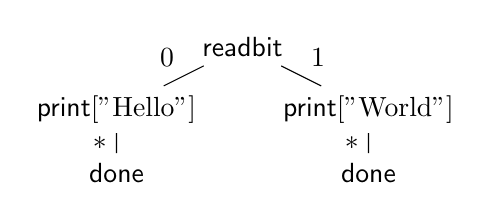
\begin{tikzpicture}[scale=0.8]
    %\node (W) at (0,0) {};
    \node (R) at (0,-1) {$\kw{readbit}$};
    \node (W0) at (-2,-2) {$\kw{print}["\text{Hello}"]$};
    \node (W1) at (+2,-2) {$\kw{print}["\text{World}"]$};
    \node (K0) at (-2,-3) {$\kw{done}$};
    \node (K1) at (+2,-3) {$\kw{done}$};
    %\path (W) edge node[auto,swap] {$*$} (R);
    \path (R) edge node[auto,swap] {0} (W0);
    \path (R) edge node[auto] {1} (W1);
    \path (W0) edge node[auto,swap] {$*$} (K0);
    \path (W1) edge node[auto,swap] {$*$} (K1);
  \end{tikzpicture}
\]
where we interpret
node labels as moves of the system,
and edge labels as moves of the environment.

%Terms are constructed by
%applying function symbols $e \in E$
%to subcomputations given for each $r \in \kw{ar}(e)$.
%In simple cases,
%the computation $e(x_r)_{r \in \kw{ar}(e)}$
%first triggers an effect $e$;
%then the context chooses $r$
%and resumes the computation as $x_r$.
%For example,
%the following effect signature
%models a very basic input/output facility:
%\[
%  E_\kw{io} :=
%    \{ \kw{readbit} : \mathbbm{2}, \:
%       \kw{writebit}[n] : \mathbbm{1} \mid
%       n \in \mathbbm{2} \}
%\]
%A computation which writes a zero,
%reads one bit, echoes its complement
%and continues as the computation $k$
%can be written as:
%\[
%  \kw{writebit}[0](
%    \kw{readbit}(
%      \kw{writebit}[1](k),
%      \kw{writebit}[0](k)))
%\]

%}}}

\begin{figure*} % fig:cal {{{
  \begin{minipage}{.9\textwidth}
    \begin{align*}
      %
      % Overlay
      %
      & \fbox{$L_\kw{bq}$} &
        S_\kw{bq} &:= V^* \\
      \kw{enq} &: V \rightarrow \mathbbm{1} &
        L_\kw{bq}.\kw{enq}(v)@\vec{q} &:= \{ * @ \vec{q} v \mid |\vec{q}| < N \} \\
      \kw{deq} &: \mathbbm{1} \rightarrow V &
        L_\kw{bq}.\kw{deq}(*)@\vec{q} &:= \{ v @ \vec{p} \: \mid \vec{q} = v \vec{p} \}
      \\[1em]
      %
      % Implementation
      %
      & \fbox{$M_\kw{bq}$} &
        R &\subseteq S_\kw{bq} \times S_\kw{rb} \\
      M_\kw{bq}.\kw{enq}(v) &:= i \leftarrow \kw{inc}_2 ; \: \kw{set}(i, v) &
        \vec{q} \mathrel{R} (f, c_1, c_2) &\Leftrightarrow
        \: c_1 < N \:\wedge\: c_2 < N \:\wedge\: {}
      \\
      M_\kw{bq}.\kw{deq}(*) &:= i \leftarrow \kw{inc}_1 ; \: \kw{get}(i) &
        & \qquad \vec{q} = f_{c_1} \cdots f_{N-1} f_0 \cdots f_{c_2}
      \\[1em]
      %
      % Underlay
      %
      & \fbox{$L_\kw{rb}$} &
        S_\kw{rb} &:= V^N \times \mathbb{N} \times \mathbb{N}
      \\
      \kw{set} &: \mathbb{N} \times V \rightarrow \mathbbm{1} &
        L_\kw{rb}.\kw{set}(i, v)@(f, c_1, c_2) &:=
        \{ *@(f', c_1, c_2) \mid i < N \wedge f' = f[i := v] \}
      \\
      \kw{get} &: \mathbb{N} \rightarrow V &
        L_\kw{rb}.\kw{get}(i)@(f, c_1, c_2) &:=
        \{ f_i@(f, c_1, c_2) \mid i < N \}
      \\
      \kw{inc}_1 &: \mathbbm{1} \rightarrow \mathbb{N} &
        L_\kw{rb}.\kw{inc}_1@(f, c_1, c_2) &:=
        \{ c_1@(f, c_1', c_2) \mid
           c_1' = (c_1 + 1) \mathop{\mathrm{mod}} N \}
      \\
      \kw{inc}_2 &: \mathbbm{1} \rightarrow \mathbb{N} &
        L_\kw{rb}.\kw{inc}_2@(f, c_1, c_2) &:=
        \{ c_2@(f, c_1, c_2') \mid
           c_2' = (c_2 + 1) \mathop{\mathrm{mod}} N \}
    \end{align*}
  \end{minipage}
  \caption{A certified abstraction layer
    $L_\kw{rb} \vdash_R M_\kw{bq} : L_\kw{bq}$
    implementing a bounded queue of size $N$
    using a ring buffer.
    The left-hand side of the figure shows
    the signatures of the overlay and underlay interfaces,
    and the code associated with the layer.
    The right-hand side shows primitive specifications
    and the simulation relation used by the correctness proof.}
  \label{fig:cal}
\end{figure*}
%}}}

\subsection{Certified abstraction layers} %{{{

To demonstrate the applicability of our results,
we will use them to construct
increasingly expressive theories of
\emph{certified abstraction layers}.
%We start with a semi-formal description,
%and will fill in the blanks as we go.
As described in \citet{popl15},
a certified abstraction layer
consists of a \emph{layer implementation} together with
two \emph{layer interfaces}:
the \emph{underlay} provides specifications for
the primitives available to the layer implementation;
the \emph{overlay} provides specifications for
the procedures which the layer implements.
A layer $M$ implementing the overlay interface $L_2$
on top of the underlay interface $L_1$ can be depicted as follows:
\[
  \begin{prooftree}
    \infer0[$L_2$]{\fbox{\qquad M \qquad}}
    \infer1[$L_1$]{}
  \end{prooftree}
\]

A layer interface $L$ has three components.
First, a \emph{signature} enumerates
primitive operations together with their types,
given as $\kw{op} : A \rightarrow B$
where $A$ and $B$ are sets.
In terms of Def.~\ref{def:esig},
this corresponds to a family $\{ \kw{op}[a] : B \mid a \in A \}$.
Second,
the set $S$ contains the \emph{abstract states} of the layer interface.
Finally, for each primitive
$\kw{op} : A \rightarrow B$,
a \emph{specification}
is given as a function:
\[
  L.\kw{op} : A \times S \rightarrow \mathcal{P}^1(B \times S) \,.
\]
Throughout the paper,
we will use $v@k \in V \times S$ to denote a pair
containing the value $v \in V$ and the state $k \in S$.
In the type of $L.\kw{op}$ above,
$\mathcal{P}^1$ corresponds to the \emph{maybe} monad:
\[
  \mathcal{P}^1(A) := \{ x \subseteq A : |x| \le 1 \} \,,
\]
where the empty set $\varnothing \in \mathcal{P}^1(A)$
serves a purpose similar to the one discussed for $\bot$
at the end of \S\ref{sec:refcal}.

%\zhong{The meaning of the empty set is very important here. We need to elaborate more.}
%\jk{I expanded on $\bot$ in 2.1 and refer to that earlier discussion here.}

As a running example,
we will use the certified layer
depicted in Fig.~\ref{fig:cal},
which implements a bounded queue with at most $N$ elements
using a circular buffer.
The underlay interface $L_\kw{rb}$
contains an array $f \in V^N$
with $N$ values of type $V$ and two counters
which will take values in the interval $0 \le c_1, c_2 < N$.
The array can be accessed through the primitives
$\kw{get}$ and $\kw{set}$;
the primitives $\kw{inc}_1$ and $\kw{inc}_2$
increment the corresponding counter
and return the counter's old value.

The overlay $L_\kw{bq}$ features two primitives
$\kw{enq}$ and $\kw{deq}$
which respectively add a new element to the queue
and remove the oldest element.
If we attempt to add an element
which would overflow the queue's capacity $N$,
or remove an element from an empty queue,
the result is $\varnothing$ (i.e., the operation aborts).

%\zhong{What does ``undefined'' mean here? the empty set?}
%\jk{Going with ``unspecified'' for now to match earlier discussion
%  of $\varnothing$}

The layer implementation $M_\kw{bq}$ 
stores the queue's elements into the array,
between the indices given by the counters' values.
This is expressed by the simulation relation $R$,
which explains how overlay states are realized by $M_\kw{bq}$ 
in terms of underlay states.
%
The code of $M_\kw{bq}$ can be interpreted in the monad
$
    S_\kw{rb} \rightarrow \mathcal{P}^1(- \times S_\kw{rb})
$,
with calls to primitives of $L_\kw{rb}$
replaced by their specifications.
We will write $M_\kw{bq}[L_\kw{rb}]$ to denote the result.
Correctness is proved by showing
for each operation
$\kw{op} \in \{ \kw{enq}(v), \kw{deq}(*) \mid v \in V \}$
the simulation:
\begin{equation}
  \label{eqn:sim}
  L_\kw{bq}.\kw{op}
  \: \mathrel{[R \rightarrow \mathcal{P}^\le({=} \times R)]} \:
  M_\kw{bq}[L_\kw{rb}].\kw{op} \,,
\end{equation}
where the relators $\rightarrow$, $\times$, $\mathcal{P}^\le$
are defined by:
\[
  \begin{array}{rclcl}
    f & [R_1 \rightarrow R_2] & g & \Leftrightarrow &
    \forall x y \bdot x \mathrel{R_1} y \Rightarrow
    f(x) \mathrel{R_2} g(y) \\
  x & [R_1 \times R_2] & y & \Leftrightarrow &
    \pi_1(x) \mathrel{R_1} \pi_1(y) \wedge
    \pi_2(x) \mathrel{R_2} \pi_2(y) \\
  s & \mathcal{P}^\le(R) & t & \Leftrightarrow &
    \forall x \in s \bdot \exists y \in t \bdot x \mathrel{R} y \,.
  \end{array}
\]
We will write $L_\kw{rb} \vdash_R M_\kw{bq} : L_\kw{bq}$
to express that condition (\ref{eqn:sim}) holds for
each operation $\kw{op}$ in the $L_\kw{bq}$ layer interface.
%\zhong{But where is $L_{rb}$ in the above condition?}
%\jk{Tried to clarify}
%Certified abstraction layers presented in this way
%can be vertically composed:
%\[
%  \begin{prooftree}
%    \hypo{L_1 \vdash_R N : L_2}
%    \hypo{L_2 \vdash_S M : L_3}
%    \infer2{L_1 \vdash_{R \circ S} M[N] : L_3}
%  \end{prooftree}
%\]

%}}}

%}}}

\section{The interaction specification monad} \label{sec:intspec} %{{{

We begin our formal development
by defining the \emph{interaction specification monad},
a variant of the free monad on an effect signature which
incorporates dual nondeterminism.

\subsection{Overview} %{{{

Given an effect signature $E$,
we construct a prefix-ordered set of plays $\bar{P}_E(A)$
corresponding to the possible interactions between
a computation with effects in $E$
and its environment,
including the computation's ultimate outcome in $A$.
The interaction specification monad $\mathcal{I}_E(A)$ is then obtained
as the free completely distributive completion of the poset $\bar{P}_E(A)$.

For each effect $e \in E$,
the interaction specification monad
has an operation
$\mathbf{I}_E^e \in \mathcal{I}_E(\kw{ar}(e))$
which triggers an instance of $e$ and returns its outcome.
Given a second effect signature $F$,
a family $(f^m)_{m \in F}$ of computations
$f^m \in \mathcal{I}_E(\kw{ar}(m))$
can be used to interpret the effects of $F$
into the signature $E$.
This is achieved by a \emph{substitution} operator $\sbt\ [f]$,
which transforms a computation $x \in \mathcal{I}_F(A)$
into the computation $x[f] \in \mathcal{I}_E(A)$,
where each occurrence of an effect $m \in F$ in $x$
is replaced by the corresponding computation $f^m$.

Effect signatures can be seen to define
particularly simple games,
and a family $(f^m)_{m \in F}$ as described above
can be interpreted as
a certain kind of strategy for the game ${!E} \multimap F$.
We use this approach to define
a first category of games and strategy specifications $\gcat^{ib}$,
where $(\mathbf{I}_E^e)_{e \in E}$ is used as
the identity morphism for $E$ and
the substitution operator is used to define composition.

%}}}

\subsection{Plays} \label{sec:intm:plays} %{{{

We first introduce the partially ordered sets of plays
which we use to construct the interaction specification monad.
Since we intend to describe \emph{active} computations,
we use \emph{odd}-length plays which start with \emph{system} moves,
by contrast with the more common approach
presented in \S\ref{sec:strat}.

\begin{definition}
The set $\bar{P}_E(A)$ of \emph{interactions}
for an effect signature $E$ and a set of values $A$
is defined inductively:
\[
  s \in \bar{P}_E(A) ::=
    \underline{v} \mid
    \underline{m} \mid
    \underline{m} n s \,,
\]
where $v \in A$, $m \in E$ and $n \in \kw{ar}(m)$.
The set $\bar{P}_E(A)$ is ordered by the prefix relation
${\sqsubseteq} \subseteq \bar{P}_E(A) \times \bar{P}_E(A)$,
defined
as the smallest relation satisfying:
\[
  \underline{v} \sqsubseteq \underline{v} \,, \qquad
  \underline{m} \sqsubseteq \underline{m} \,, \qquad
  \underline{m} \sqsubseteq \underline{m} n t \,, \qquad
  \begin{prooftree}
    \hypo{s \sqsubseteq t}
    \infer1{\underline{m} n s \sqsubseteq \underline{m} n t}
  \end{prooftree} \,.
\]
\end{definition}

A play corresponds to a finite observation of
an interaction between the system and the environment.
At any point in such an interaction,
the system can terminate the interaction with a given value ($v$),
or it can trigger an effect $m \in E$ and
wait to be resumed by
an answer $n \in \kw{ar}(m)$ of the environment
($\underline{m} n s$).

A play which concludes before
the environment answers a query from the system ($\underline{m}$)
denotes that no information has been observed after that point.
It can be refined by a longer observation
of an interaction which begin with the same sequence of
questions and answers.

%
%\zhong{Add a comment why the play here is odd length but the one
%  in Section 2.2 is even length.}
%\jk{There is a comment before the definition but we could move it
%  if needed, and possibly draw the contrast with 2.2 more explicitly}
%

%}}}

\subsection{Interaction specifications} %{{{

We define our monad as the free completely distributive completion
of the corresponding poset of plays.

For the sake of conciseness and clarity,
we will use the order embedding associated with $\mathbf{FCD}$
implicitly,
so that an element of a poset $s \in P$
can also be regarded as an element of
its completion $s \in \mathbf{FCD}(P)$.
Likewise,
for a completely distributive lattice $L$,
we can implicitly
promote a monotonic operator
$f : P \rightarrow L$
to its extension
$f : \mathbf{FCD}(P) \rightarrow L$
as given by the universal property of
the free completely distributive lattice completion of $P$.
These conventions are at work
in the following definition.

\begin{definition} \label{def:intm} % Interaction specification monad {{{
The \emph{interaction specification monad}
for an effect signature $E$
maps a set of values $A$
to the free completely distributive completion
of the corresponding plays:
\[
    \mathcal{I}_E(A) :=
      \mathbf{FCD}(\bar{P}_E(A))
\]
An element $x \in \mathcal{I}_E(A)$ is called
an \emph{interaction specification}.

The monad's action on a function $f : A \rightarrow B$
replaces the values in
an interaction specification with their image by $f$:
\begin{align*}
  \mathcal{I}_E(f)(\underline{v}) &:= \underline{f(v)} \\
  \mathcal{I}_E(f)(\underline{m}) &:= \underline{m} \\
  \mathcal{I}_E(f)(\underline{m} n s) &:=
    \underline{m} n \, \mathcal{I}_E(f)(s) \,.
\end{align*}
The monad's unit
$\eta^E_A : A \rightarrow \mathcal{I}_E(A)$
is the embedding of a single play
consisting only of the given value:
\[
    \eta^E_A(v) := \underline{v}
\]
Finally, the multiplication
$\mu^E_A : \mathcal{I}_E(\mathcal{I}_E(A)) \rightarrow \mathcal{I}_E(A)$
carries out the outer computation and
sequences it with any computation it evaluates to:
\begin{align*}
  \mu^E_A(\underline{x}) &:= x \\
  \mu^E_A(\underline{m}) &:= \underline{m} \\
  \mu^E_A(\underline{m} n s) &:=
    \underline{m} \sqcup \underline{m} n \, \mu^E_A(s) \,.
\end{align*}
\end{definition}

%\zhong{What are you proving here? please state the theorem explicitly.}
%\jk{Added a sentence at the beginning}
%
%\begin{proof} %{{{
We can verify as follows that
$(\mathcal{I}_E, \eta_E, \mu_E)$
does define a monad.
From the definitions above and
the fact that $\mathbf{FCD}$ is itself a monad,
we can show that
for all functions $f : A \rightarrow B$,
\[
    \eta^E_B \circ f = \mathcal{I}_E(f) \circ \eta^E_A \,.
\]
By inductions on plays, we can also show that:
\[
    \mu^E_B \circ \mathcal{I}_E(\mathcal{I}_E(f)) =
      \mathcal{I}_E(f) \circ \mu^E_A \,.
\]
This establishes that $\eta^E$ and $\mu^E$
are natural transformations.
By a similar approach,
we can show for a set $X$ that:
\begin{align*}
  \mu^E_X \circ \mathcal{I}_E(\mu^E_X) &=
    \mu^E_X \circ \mu^E_{\mathcal{I}_E(X)} \\
  \mu^E_X \circ \mathcal{I}_E(\eta^E_X) &=
    \mu^E_X \circ \eta^E_{\mathcal{I}_E(X)} \,.
\end{align*}
%\end{proof}
%}}}

%}}}

The most subtle aspect of Def.~\ref{def:intm}
is the case for $\mu^E_A(\underline{m} n s)$,
which includes $\underline{m}$ as well as $\underline{m} n \mu^E_A(s)$.
This is both
to ensure that the effects of the first computation are preserved
when the second computation is undefined, and
to ensure the monotonicity of the underlying function
used to define $\mu^E_A$.
Consider for example
$\underline{m} n \underline{\bot} \in \bar{P}_E(\mathcal{I}_E(A))$.
The $\mathbf{FCD}$ extension
of the function $s \mapsto \underline{m} n s$
preserves $\bot$,
with the consequence that
$\underline{m} = \mu^E_A(\underline{m}) \nsqsubseteq
 \underline{m} n \mu^E_A(\underline{\bot}) = \bot$,
even though
$\underline{m} \sqsubseteq \underline{m} n \underline{\bot}$.

As usual,
the Kleisli extension of a function $f : A \rightarrow \mathcal{I}_E(B)$
is the function $f^* = \mu^E_B \circ \mathcal{I}_E(f)$.
We extend the notations used for $\mathbf{FCD}$
to the monad $\mathcal{I}_E$.

%Given directly:
%\begin{align*}
%  f^\dagger(\underline{v}) &:= f(v) \\
%  f^\dagger(\underline{m}) &:= \underline{m} \\
%  f^\dagger(\underline{m} n s) &:=
%    \underline{m} \sqcup \underline{m} n f^\dagger(s)
%\end{align*}

%}}}

\subsection{Interaction primitives} %{{{

The operations of an effect signature $E$
can be promoted to interaction specifications of $\mathcal{I}_E$
as follows.

\begin{definition}[Interaction primitive]
For an effect signature $E$ and
an operation $m \in E$,
the interaction specification
$\mathbf{I}_E^m \in \mathcal{I}_E(\kw{ar}(m))$
is defined as:
\[
  \mathbf{I}_E^m :=
    \bigsqcup_{n \in \kw{ar}(m)} \underline{m} n \underline{n}
\]
%If the context permits,
%we can write $\mathbf{I}_E^m$ simply as $m$.
%\jk{does that ever actually happen?}
\end{definition}
Note that in the play $\underline{m} n \underline{n}$,
the first occurrence of $n$ is the environment's answer,
whereas the second occurrence is the value returned by $\mathbf{I}_E^m$.

To model effect handling for a signature $F$,
we use a family of interaction specifications
$(f^m)_{m \in F}$
to provide an interpretation $f^m \in \mathcal{I}_E(\kw{ar}(m))$
of each effect $m \in F$
in terms of another effect signature $E$.
This allows us to transform an interaction specification
$x \in \mathcal{I}_F(A)$
into an interaction specification
$x[f] \in \mathcal{I}_E(A)$,
defined as follows.
The constructions $\bot$ and $\{P\}$ were discussed in \S\ref{sec:refcal};
they carry similar meanings in the context of the
interaction specification monad.

\begin{definition}[Interaction substitution]
Given the effect signatures $E, F$ and the set $A$,
for an interaction specification $x \in \mathcal{I}_F(A)$
and a family $(f^m)_{m \in F}$ with $f^m \in \mathcal{I}_E(\kw{ar}(m))$,
the \emph{interaction substitution} $x[f] \in \mathcal{I}_E(A)$
is defined by:
\begin{align*}
  \underline{v}[f] &:= \underline{v} \\
  \underline{m}[f] &:= r \leftarrow f^m ; \bot \\
  \underline{m}ns[f] &:= r \leftarrow f^m ; \{r = n\} ; s[f] \,.
\end{align*}
\end{definition}

%\zhong{Where is the definition of $\bot$?}
%\jk{Now addressed in \S2.1 and in the sentence preceding the definition}

The outcome of the interaction specification is left unchanged,
but effects are replaced by their interpretation.
Whenever that interpretation produces an outcome $r$,
the substitution process resumes with the remainder of any
matching plays of the original computation.

%}}}

\subsection{Categorical structure} \label{sec:intm:cat} %{{{

As presented so far,
the interaction specification monad
can be seen as an extension of the refinement calculus
able to model effectful computations
for a given signature.
We now shift our point of view to game semantics
and show how interaction substitutions
can be used to define a simple category of games and strategies
featuring dual nondeterminism and alternating refinement.

\begin{definition}[Interaction substitutions as morphisms]
Consider the effect signatures $E$, $F$ and $G$.
We will write $f : E \rightarrow F$
whenever $(f^m)_{m \in F}$ is a family of interactive computations
such that $f^m \in \mathcal{I}_E(\kw{ar}(m))$.
Then for $f : E \rightarrow F$ and $g : F \rightarrow G$,
we define $g \circ f : E \rightarrow G$ as:
\[ (g \circ f)^m = g^m[f] \,. \]
The completely distributive lattice structure
of $\mathcal{I}_F(-)$ can be extended pointwise
to interaction substitutions,
so that for a family $(f_i)_{i \in I}$
with $f_i : E \rightarrow F$,
we can define the substitutions
$(\bigsqcup_{i \in I} f_i) : E \rightarrow F$ and
$(\bigsqcap_{i \in I} f_i) : E \rightarrow F$,
%as:
%\begin{gather*}
%    \left( \bigsqcup_{i \in I} f_i \right)^m :=
%      \bigsqcup_{i \in I} f_i^m \qquad
%    \left( \bigsqcap_{i \in I} f_i \right)^m :=
%      \bigsqcap_{i \in I} f_i^m \,,
%\end{gather*}
and for $f, g : E \rightarrow F$
we can define refinement as:
\[
    f \sqsubseteq g \: \Leftrightarrow \:
    \forall m \in F \bdot f^m \sqsubseteq g^m \,.
\]
\end{definition}

An interaction substitution $f : E \rightarrow F$
can be interpreted as a \emph{well-bracketed} strategy for the game
${!E} \multimap F$.
In this game,
the environment first plays a move $m \in F$.
The system can then ask a series of questions
$q_1, \ldots q_k \in E$
to which the environment will reply with
answers $r_i \in \kw{ar}(q_i)$,
and finally produce an answer $n \in \kw{ar}(m)$
to the environment's initial question $m$.
The plays of ${!E} \multimap F$
are restricted to a single top-level question $m$.
In addition, the well-bracketing requirement
imposes that at any point,
only the most recent pending question
may be answered.

Compared with the usual notion of strategy,
our model introduces arbitrary demonic choices and
relaxes constraints over angelic choices.
%Specifically,
%plays which first differ in a system move
%are allowed to coexist
%both angelically and demonically.
The definition of $g \circ f$ given above
otherwise corresponds to the traditional
definition of strategy composition.
The identity strategy is given by $\mathbf{I}_E : E \rightarrow E$.

\begin{lemma}
Consider the effect signatures $E, F, G, H$ and
the substitutions
$f : E \rightarrow F$,
$g : F \rightarrow G$ and
$h : G \rightarrow H$.
The following properties hold:
\begin{gather*}
  \mathbf{I}_F \circ f = f \circ \mathbf{I}_E = f \\
  h \circ (g \circ f) = (h \circ g) \circ f
\end{gather*}
Composition preserves all extrema on the left,
and all non-empty extrema on the right.
\begin{proof}
Using properties of $\mathbf{FCD}$
and inductions on plays.
\end{proof}
\end{lemma}

Having established the relevant properties,
we can now define our first category of games and strategies.

\begin{definition}
The category $\gcat^{ib}$ has effect signatures as objects
and interaction substitutions as morphisms.
The hom-sets $\gcat^{ib}(E, F)$
are completely distributive lattices,
with composition preserving all extrema on the left,
and all non-empty extrema on the right.
\end{definition}

%}}}

\subsection{Products} %{{{

Effect signatures can be combined in the following way.

\begin{definition}
We define the effect signature
$1 := \varnothing$.
For a family of effect signatures $(E_i)_{i \in I}$,
we define:
\[
  \bigotimes_i E_i := \{ (i, e) : \kw{ar}(e) \mid i \in I, e \in E_i \}
\]
\end{definition}

For example,
the signature $E_\kw{io}$ above is equivalent
to the following composite one:
\[
    \{ \kw{readbit} : \mathbbm{2} \} \otimes
    \{ \kw{print}[s] : \mathbbm{1} \mid s \in \kw{string} \} \otimes
    \{ \kw{done} : \varnothing \}
\]

The construction $\otimes$ gives products in the category $\gcat^{ib}$,
as demonstrated below.

\begin{theorem}
The category $\gcat^{ib}$ has all products.
Objects are given by $\bigotimes_{i \in I} E_i$
and projection arrows are
given for each $i \in I$ by
the interaction substitution:
\begin{gather*}
    \pi_i : \bigotimes_{j \in I} E_j \rightarrow E_i \qquad
    \pi_i^m := (i, m) \,.
\end{gather*}
\begin{proof}
\jk{Remove?}
We need to show that for an effect signature $X$
and a collections of substitutions $(f_i)_{i \in I}$ with
$f_i : X \rightarrow E_i$,
there is a unique
$\langle f_i \rangle_{i \in I} : X \rightarrow \bigotimes_{i \in I} E_i$
such that for all $i \in I$:
\[
    f_i = \pi_i \circ \langle f_j \rangle_{j \in I} \,.
\]
Note that for $x : X \rightarrow \bigotimes_{i \in I} E_i$,
$i \in I$ and $m \in E_i$, we have:
\[
    (\pi_i \circ x)^m = \pi_i^m[x] = (i, m) [x] = x^{(i, m)}
\]
Hence, $\langle f_i \rangle_{i \in I}$ is uniquely defined as:
\[
    \langle f_i \rangle_{i \in I}^{(j, m)} := f_j^m \,.
\]
\end{proof}
\end{theorem}

%}}}

\subsection{Certified abstraction layers} \label{sec:intspec:cal} %{{{

Certified abstraction layers can be embedded into
the category $\gcat^{ib}$ as follows.

%\paragraph{Signatures}

The signature of a layer interface or implementation
can be encoded as an effect signature.
For example:
\begin{align*}
  E_\kw{bq} &:= \{
    \kw{enq}[v] : \mathbbm{1}, \kw{deq} : V \mid
    v \in V \} \\
  E_\kw{rb} &:= \{
    \kw{set}[i, v] \! : \! \mathbbm{1},
    \kw{get}[i] \! : \! V,
    \kw{inc}_1 \! : \! \mathbb{N},
    \kw{inc}_2 \! : \! \mathbb{N} \! \mid \!
    i \in \mathbb{N}, v \in V \}
\end{align*}
A layer implementation $M$ with
an underlay signature $E$ and
an overlay signature $F$
can then be interpreted as a morphism
$\llbracket M \rrbracket : E \rightarrow F$
in a straightforward manner,
by interpreting underlay operations
used in the definition of $M$
by the corresponding interaction primitives:
\[
  \llbracket M \rrbracket^m := (M.m)[e := \mathbf{I}_E^e]_{e \in E}
\]

\paragraph{Interfaces}
In order to handle the layer's abstract data,
we can extend signatures with state in the following way:
\[
  E@S :=
    \{ m@k : \kw{ar}(m) \times S \mid
       m \in E, k \in S \}
\]
A layer interface $L$ with a signature $E$
and states in $S$
can be interpreted as
a morphism $\llbracket L \rrbracket : 1 \rightarrow E@S$
almost directly,
mapping $\varnothing$ to $\bot$
in outcomes of primitive specifications:
\[
  \llbracket L \rrbracket^{m@k} :=
    \bigsqcup L.m@k
\]

\paragraph{Keeping state}
For a morphism $f : E \rightarrow F$,
we construct $f@S : E@S \rightarrow F@S$
which keeps updating a state $k \in S$
as it performs effects in $E@S$,
then adjoins the final state to any answer
returned by $f$.
We define
$-\#- : \bar{P}_E \times S \rightarrow \mathcal{I}_{E@S}(A \times S)$:
\begin{align*}
  \underline{v}\#k &:= \underline{v@k} \\
  \underline{m}\#k &:= \underline{m@k} \\
  \underline{m}ns\#k &:=
    \bigsqcup_{k' \in S} \, \underline{m@k} \,\, n@k' \, s\#k' \,,
\end{align*}
and extend it to morphisms as $(f@S)^{m@k} := f^m\#k$.
Then in particular,
running a layer implementation
$\llbracket M \rrbracket : E \rightarrow F$
on top of a layer interface
$\llbracket L \rrbracket : 1 \rightarrow E@S$
yields the morphism
$\llbracket M \rrbracket @ S \circ \llbracket L \rrbracket :
 1 \rightarrow F@S$.

\paragraph{Simulation relations}

The most interesting aspect of our embedding
is the representation of simulation relations.
We will see that dual nondeterminism
allows us to represent them as regular morphisms.

Recall the definition of
the judgment $L_1 \vdash_R M : L_2$,
which means that a layer implementation $M$
correctly implements $L_2$ on top of $L_1$
through a simulation relation $R \subseteq S_2 \times S_1$.
If we write $L_1'$ for the layer interface obtained
by interpreting $M$ on top of $L_1$,
then:
\[
  L_1 \vdash_R M : L_2 \:\Leftrightarrow\:
  \forall m \in E_2 \bdot
    L_2^m
    \mathrel{[R \rightarrow \mathcal{P}^\le({=} \times R)]}
    {L_1'}^m
\]
We will use the families of morphisms
$R^*_E : E@S_2 \rightarrow E@S_1$ and
$R_*^E : E@S_1 \rightarrow E@S_2$
to encode this judgment:
\[
  {\everymath={\displaystyle}
  \begin{array}{r@{\:}c@{\:}c@{\:}c@{\:}l}
  (R^*_E)^{m@k_1} := &
    \bigsqcup_{k_2 \in R^{-1}(k_1)} &
    \bigsqcup_{k_2' \in S_2} &
    \bigsqcap_{k_1' \in R(k_2')} &
    \: \underline{m@k_2} \: n@k_2' \: \underline{n@k_1'} \\
  (R_*^E)^{m@k_2} := &
    \bigsqcap_{k_1 \in R(k_2)} &
    \bigsqcup_{k_1' \in S_1} &
    \bigsqcup_{k_2' \in R^{-1}(k_1')} &
    \: \underline{m@k_1} \: n@k_1' \: \underline{n@k_2'}
  \end{array}}
\]
They yield two equivalent ways to encode
layer correctness as refinement properties.

In the first case,
$R^*_E$ is intended to translate
a high-level specification $\sigma$
which uses overlay states $k_2, k_2' \in S_2$
into a low-level specification $R^*_E \circ \sigma$
which uses underlay states
$k_1, k_1' \in S_1$.
The client calls $R^*_E$
with an underlay state $k_1$,
with the expectation that if there is \emph{any}
corresponding overlay state,
then $R^*_E \circ \sigma$ will behave accordingly
(it is angelic with respect to its choice of $k_2$).
On the other hand,
$R^*_E \circ \sigma$ is free to choose any underlay representation
$k_1'$
for the outcome $k_2'$ produced by $\sigma$,
and the client must be ready to accept it
(it is demonic with respect to its choice of $k_1'$).

In the second case,
$R_*^E \circ \tau$ is intended as
the strongest high-level specification
which a low-level component $\tau$ implements
with respect to $R$.
For an overlay state $k_2 \in S_2$,
$\tau$ may behave in various ways
depending on the corresponding underlay state $k_1 \in S_1$
it is invoked with,
and so the specification must allow them using demonic choice.
On the other hand,
when $\tau$ returns with a new underlay state $k_1'$,
the environment is free to choose
how to interpret it as an overlay state $k_2'$.

%\begin{lemma}
%Given the relation $R \subseteq S_1 \times S_2$,
%the effect signatures $E, F$, and
%the morphisms
%$\sigma : E \rightarrow F@S_1$ and
%$\tau : E \rightarrow F@S_2$,
%the following property holds:
%\[
%  R^*_F \circ \sigma \sqsubseteq \tau
%  \Leftrightarrow
%  \sigma \sqsubseteq R_*^F \circ \tau
%\]
%\end{lemma}

\begin{theorem}
Define
$\sigma := \llbracket L_2 \rrbracket$ and
$\tau := \llbracket M \rrbracket @ S_1 \circ \llbracket L_1 \rrbracket$.
Then:
\[
  R^*_{E_2} \!\circ \sigma \sqsubseteq \tau
  \: \Leftrightarrow \:
  L_1 \vdash_R M : L_2
  \: \Leftrightarrow \:
  \sigma \sqsubseteq R_*^{E_2} \!\circ \tau \,.
\]
\begin{proof}
The proof is straightforward but requires
Thm.~5.3 from \citet{dndf}.
\end{proof}
\end{theorem}

%\zhong{Should there be a $\sigma$ somewhere above instead of having $\tau$ twice?}
%\jk{Those are the same, but I renamed for clarity}

%}}}

%}}}

\section{Stateful and reentrant strategies} \label{sec:gamesem} %{{{

% Preamble {{{

As discussed in \S\ref{sec:intm:cat}
the morphisms of $\gcat^{ib}(E, F)$
correspond to well-bracketed strategies
for the game ${!E} \multimap F$.
%By the \emph{bang lemma} given in \cite{gamesem99},
%they also corresponds to the
Equivalently, they correspond to
\emph{innocent} well-bracketed strategies
for the game ${!E} \multimap {!F}$.

In this section,
we sketch a more general model
which relaxes this innocence constraint,
allowing strategies to retain state
across different activations.
We explain how the new model $\gcat^b$ can embed
the morphisms of $\gcat^{ib}$,
and how it can be used to characterize
certified abstraction layers
independently of the states used in their description.

%}}}

\subsection{Overview} %{{{
\label{sec:arrow}

The game ${!E} \multimap {!F}$
proceeds similarly to ${!E} \multimap F$,
but instead of playing a single instance of $F$,
the environment is free to initiate a new instance
whenever it is in control,
by asking a new top-level question $m \in F$.
This can happen as the initial move,
after the system asks a question in ${!E}$,
or after the system answers
a question of the environment in ${!F}$.

%The system's own questions in ${!E}$
%are made in the context of a specific question in ${!F}$.
%this information is often encoded using \emph{justification pointers},
%whereby all non-top-level moves are required to refer to
%an earlier move,
%in a way that is compatible with the enabling relation
%used to define the game's arena.
%The well-bracketing condition only allows the players
%to answer the most recent pending question.
%ask new questions in the context of
%the most recent pending question.
%In our limited setting,
%the innocence condition requires that the system
%behave in the same way for each top-level question.

%To specify an innocent strategy
%for our game ${!E} \multimap {!F}$,
%it is enough to specify its behavior
%for a single question of $F$:
%the behavior of the full strategy can be reconstructed
%by duplicating this behavior whenever needed.
%This is traditionally expressed as a promotion operator
%mapping a strategy $\sigma : {!A} \multimap B$
%to the strategy $\sigma^\dagger : {!A} \multimap {!B}$.

%In the game ${!E} \multimap {!F}$,
%when the system asks a question in ${!E}$,
%the environment may delay its answer
%and instead ask a new question of its own in ${!F}$.
%Since we only consider well-bracketed strategies,
%such ``reentrant'' questions must be answered by the system
%before then environment can answer the original one.

The well-bracketing requirement only allows the players
to answer the most recent pending question.
%In the context of ${!E} \multimap {!F}$,
It enforces a kind of \emph{stack discipline}
on the succession of questions and answers.
A well-bracketed play
can be interpreted as an activation tree,
where questions are understood as function calls
between the system and the environment,
and answers are understood as the
corresponding calls returning.
%The stack discipline is enforced by the fact that
%questions must be answered in the reverse order
%in which they were asked.
%The alternation constraint
%corresponds to the sequential nature of the computation.

%}}}

\subsection{Games} %{{{

To facilitate reasoning,
and make it easier to describe operators on strategies
in a systematic way,
we describe games as a specific kind of graph
where vertices represent players
and edges represent questions that can be asked
by one player to another.
%Operations on plays and strategies
%can then be specified in terms of
%their action on individual questions.
Generalizing from effect signatures,
questions are assigned an arity
which gives the type of the answer.

\begin{definition}
A \emph{game signature} $\Gamma$
is a set of players with a distinguished element $\kw{O}$,
together with an effect signature $\Gamma(u, v)$
for all $u, v \in \Gamma$.
The operations $m \in \Gamma(u, v)$ are called
the \emph{questions} of $u$ to $v$,
and the elements $n \in \kw{ar}(m)$ are called
\emph{answers} to the question $m$.
\end{definition}

We depict game signatures as directed graphs
whose vertices are the players and
whose edges are labeled by the corresponding effect signature.
Missing edges correspond to the empty signature $\varnothing$.
For example,
%an effect signature $E$ corresponds to
%the single-player game signature:
%\[
%  [E] =
%  \begin{tikzpicture}[baseline=(O.base)]
%    \node[circle,double,draw] (O) at (0,0) {$\kw{O}$};
%    \path[->] (O) edge[loop right] node[auto] {E} (O);
%  \end{tikzpicture} \,,
%\]
%and
the game ${!E} \multimap {!F}$ is generated by
the game signature:
\[
  [E,F] =
  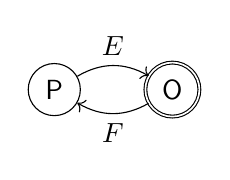
\begin{tikzpicture}[baseline=(O.base),scale=1.5]
    \node[circle,draw,double] (O) at (0,0) {$\kw{O}$};
    \node[circle,draw] (P) at (-1,0) {$\kw{P}$};
    \path[->] (P) edge[bend left] node[above] {$E$} (O);
    \path[->] (O) edge[bend left] node[below] {$F$} (P);
  \end{tikzpicture}
\]
When we consider the ways in which questions propagate
through a game signature, % system such as the one above,
the distinguished player $\kw{O}$ serves the role
of both a source and sink.
As such, it is visually useful
to depict $\kw{O}$ as two nodes,
one capturing the incoming edges of $\kw{O}$, and
one capturing its outgoing edges.
For example,
the following game signature
generates the interaction sequences
used in the definition of
strategy composition:
\[
  [E,F,G] =
  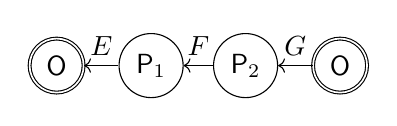
\begin{tikzpicture}[baseline=(O1.base),scale=1.2]
    \node[circle,double,draw] (O1) at (0,0) {$\kw{O}$};
    \node[circle,draw] (P1) at (-1,0) {$\kw{P}_2$};
    \node[circle,draw] (P2) at (-2,0) {$\kw{P}_1$};
    \node[circle,double,draw] (O2) at (-3,0) {$\kw{O}$};
    \path[->] (O1) edge node[above] {$G$} (P1);
    \path[->] (P1) edge node[above] {$F$} (P2);
    \path[->] (P2) edge node[above] {$E$} (O2);
  \end{tikzpicture}
\]

As another example of a game signature,
a situation where
$\sigma_1 : E_1 \rightarrow F_1$ and
$\sigma_2 : E_2 \rightarrow F_2$
interact with the environment
independently of one another
can be described as:
\[
  [E_1,F_1] \vee [E_2,F_2] =
  \begin{tikzpicture}[baseline=(O.base),xscale=1.2]
    \node[circle,draw,double] (O1) at (+1,0) {$\kw{O}$};
    \node[circle,draw,double] (O2) at (-1,0) {$\kw{O}$};
    \node[circle,draw] (P1) at (0,+0.5) {$\kw{P}_1$};
    \node[circle,draw] (P2) at (0,-0.5) {$\kw{P}_2$};
    \path[->] (O1) edge node[auto=right] {$F_1$} (P1);
    \path[->] (P1) edge node[auto=right] {$E_1$} (O2);
    \path[->] (O1) edge node[auto=left] {$F_2$} (P2);
    \path[->] (P2) edge node[auto=left] {$E_2$} (O2);
  \end{tikzpicture}
\]
The signature above will be used to compute
tensor products of strategies.
These constructions generalize as follows.

\begin{definition}[Constructions on game signatures]
For a collection of effect signature $(E_i)_{1 \le i \le n}$
and an effect signature $F$,
the game signature $[ E_1, \ldots, E_n, F ]$
has the players
$\kw{O}, \kw{P}_1, \ldots, \kw{P}_n$
and the following edges:
\[
  [E_1, \ldots, E_n, F] :=
  \begin{tikzpicture}[scale=1.2,baseline=(O.base)]
    \node[circle,draw,double] (O1) at (0,0) {$\kw{O}$};
    \node[circle,draw] (P1) at (1,0) {$\kw{P}_1$};
    \node (D) at (2,0) {$\ldots$};
    \node[circle,draw] (Pn) at (3,0) {$\kw{P}_n$};
    \node[circle,draw,double] (O2) at (4,0) {$\kw{O}$};
    \path[->] (P1) edge node[above] {$E_1$} (O1);
    \path[->] (D) edge node[above] {$E_2$} (P1);
    \path[->] (Pn) edge node[above] {$E_n$} (D);
    \path[->] (O2) edge node[above] {$F$} (Pn);
  \end{tikzpicture}
\]
For a collection of game signatures $(\Gamma_i)_{i \in I}$,
the \emph{wedge sum} $\bigvee_{i \in I} \Gamma_i$ has the players:
\[
    \{ \kw{O} \} \cup
    \{ (i, p) \mid i \in I \wedge p \in \Gamma_i \setminus \{ \kw{O} \} \}
\]
For $i \in I$ and $p \in \Gamma_i$, the corresponding player in
$\bigvee_{j \in I} \Gamma_j$ is:
\[
  \iota_i(p) := \begin{cases}
    \kw{O} & \text{if } p = \kw{O} \\
    (i, p) & \text{otherwise.}
  \end{cases}
\]
Then for each question $m : u \rightarrow v$ in $\Gamma_i$,
the wedge sum has a corresponding question
$\iota_i(m) : \iota_i(u) \rightarrow \iota_i(v)$.
\end{definition}

%Note that the empty game signature $0$ can be
%described in the following way:
%\[
%  0 := \bigvee \varnothing =
%  \begin{tikzpicture}[baseline=(O.base)]
%    \node[circle,draw,double] {$\kw{O}$};
%  \end{tikzpicture}
%\]

%}}}

\subsection{Plays and strategies} %{{{

The description of the game ${!E} \multimap {!F}$
using the game signature $[E, F]$
already encodes the alternating aspect of plays.
The well-bracketed plays and strategies
over a game signature
can be described as follows.

At any point in a play over a signature $\Gamma$,
its possible evolutions
are characterized by the stack of pending questions.

\begin{definition}
For a game signature $\Gamma$ and a player $p \in \Gamma$,
a \emph{$p$-stack} over $\Gamma$ is a path:
\[
  \kw{O} = p_0 \xrightarrow{m_1} p_1 \xrightarrow{m_2} \cdots
             \xrightarrow{m_n} p_n = p
\]
where $p_i \in \Gamma$ and $m_i \in \Gamma(p_{i-1}, p_i)$.
We will write this path as
$\kappa = m_1' \cdots m_n' : \kw{O} \twoheadrightarrow p 
 \in \Gamma$.
\end{definition}

Such stacks can in turn be arranged in a graph $\hat{\Gamma}$
over which the game associated with $\Gamma$ will be played.

\begin{definition}[Strategy specifications] %{{{
For a signature $\Gamma$,
the graph $\hat{\Gamma}$ is defined as follows.
The vertices of $\hat{\Gamma}$ are pairs $(u, \kappa)$
in which $u \in \Gamma$ and $\kappa$ is a $u$-stack.
For each question $m \in \Gamma(u,v)$
and stack $\kappa : \kw{O} \twoheadrightarrow u$,
there is an edge:
\[
    m : (u, \kappa) \rightarrow (v, \kappa m) \in \hat{\Gamma} \,.
\]
In addition, for each answer $n \in \kw{ar}(m)$,
there is an edge:
\[
    n : (v, \kappa m) \rightarrow (u, \kappa) \in \hat{\Gamma} \,.
\]
The \emph{plays} over $\Gamma$
are paths of type
$(\kw{O}, \epsilon) \twoheadrightarrow (\kw{O}, \kappa)
 \in \hat{\Gamma}$,
where $\kappa : \kw{O} \twoheadrightarrow \kw{O} \in \Gamma$
is a stack.
We will write
$P \, \Gamma$
for the poset of plays over $\Gamma$
under the prefix ordering.
The \emph{strategy specifications} for $\Gamma$
are given by the completion:
\[
    S \, \Gamma := \mathbf{FCD}(P \, \Gamma) \,.
\]
\end{definition}
%}}}

%}}}

\subsection{Operations on strategies} %{{{

\begin{definition}
A \emph{transformation}
from the game signature $\Gamma_1$
to the game signature $\Gamma_2$
associates to each player $p \in \Gamma_1$ a player $f(p) \in \Gamma_2$
with $f(\kw{O}) = \kw{O}$,
and to each question $m \in \Gamma_1(u,v)$
a \emph{path} of questions in $\Gamma_2$:
\[
  f(u) = p_0 \xrightarrow{m_1'} p_1 \xrightarrow{m_2'} \cdots
             \xrightarrow{m_n'} p_n = f(v) \,,
\]
written as
$f(m) = m_1' m_2' \cdots m_n' : f(u) \twoheadrightarrow f(v)$, and
such that
$\kw{ar}(m_1') = \cdots = \kw{ar}(m_n') = \kw{ar}(m)$.
We extend $f$ itself to the paths in $\Gamma_1$
by taking the image of $m_1 \cdots m_n : u \twoheadrightarrow v$
to be:
\[
  f(m_1 \cdots m_n) := f(m_1) \cdots f(m_n) :
    f(u) \twoheadrightarrow f(v) \,.
\]
We write $\mathbf{GST}$ for the category of
game signatures and transformations.
\end{definition}

In other words,
a transformation
is a structure-preserving map on paths.
Transformations can be extended to plays.

\begin{definition}[Action on plays]
A transformation
$f : \Gamma_1 \rightarrow \Gamma_2$
induces a monotonic function
$P f  : P \, \Gamma_1 \rightarrow P \, \Gamma_2$
as follows.
For $m \in \Gamma(u, v)$ and $\kappa : \kw{O} \twoheadrightarrow u$,
the image of the move
$m : (u, \kappa) \rightarrow (v, \kappa m)$
is the path:
\[
 f(m) : (f(u), f(\kappa)) \twoheadrightarrow
        (f(v), f(\kappa) f(m)) \,.
\]
For $n \in \kw{ar}(m)$,
the image of
$n : (v, \kappa m) \rightarrow (u, \kappa)$
is the path:
\[
 n^{|f(m)|} : (f(v), f(\kappa) f(m)) \twoheadrightarrow
              (f(u), f(\kappa)) \,,
\]
where $n^{|f(m)|}$ denotes a sequence $nn \cdots n$
of copies of the answer $n \in \kw{ar}(m)$
of same length as the path $f(m)$.
\end{definition}

Operators on strategies will generally be defined
by a game signature of global \emph{interaction sequences},
and will use transformations to project out
the corresponding plays of the arguments and the result.

\paragraph{Composition} %{{{

When composing the strategy specifications
$\sigma \in S \, [E, F]$ and
$\tau \in S \, [F, G]$
to obtain $\tau \circ \sigma \in S \, [E, G]$,
we will use the transformation
$\psi^c_X : [E,F,G] \rightarrow [E,G]$
to describe the externally observable behavior
of interaction sequences in $[E,F,G]$:
\begin{gather*}
  \psi^c_X(\kw{P}_1) = \psi^c_X(\kw{P}_2) = \kw{P} \qquad
  \psi^c_X(\kw{O}) = \kw{O}
  \\
  \psi^c_X(m) = \begin{cases}
    \epsilon & \text{if } m \in F \\
    m & \text{otherwise}
  \end{cases}
\end{gather*}
This can be described concisely as
$\psi^c_X = [1,0,1]$,
with:
\begin{align*}
  \psi^c_1 &:= [1,1,0] :
    [E,F,G] \rightarrow [E,F] \\
  \psi^c_2 &:= [0,1,1] :
     [E,F,G] \rightarrow [F,G]
\end{align*}
defined similarly.

We can now formulate the composition of strategy specifications as follows.
The ``footprint'' of the plays $s_1 \in P \, [E,F]$ and $s_2 \in P \, [F,G]$
can be defined as:
\[
  \psi^c(s_1, s_2) :=
    \bigsqcup_{s \in P [E,F,G]}
    \{ \psi^c_1(s) \sqsubseteq s_1 \wedge \psi^c_2(s) \sqsubseteq s_2 \} ;
    \psi^c_X(s) \,.
\]
In other words,
the angel chooses a global play $s$
matching $s_1$ and $s_2$
and produces its external view.
By extending $\psi^c$ to strategy specifications
in the expected way, we obtain:
\[
  \tau \circ \sigma = 
    s \leftarrow \sigma ;
    t \leftarrow \tau ;
    \psi^c(s, t) \,.
\]

%}}}

\paragraph{Identity} %{{{

The strategy $\mathrm{id}_E \in S \, [E,E]$
uses the signature:
\[
  [E] =
  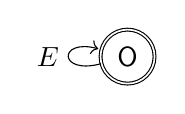
\begin{tikzpicture}[baseline=(O.base)]
    \node[circle,draw,double] (O) at (0,0) {$\kw{O}$};
    \path[->] (O) edge[loop left] node[auto] {$E$} (O);
  \end{tikzpicture}
\]
and the transformation:
\begin{gather*}
  \psi^\mathrm{id}_X := [2] : [E] \rightarrow [E,E] \\
  \psi^\mathrm{id}_X(\kw{O}) := \kw{O} \qquad
  \psi^\mathrm{id}_X(m) := mm
\end{gather*}
Then $\mathrm{id}_E$ is defined as:
\[
  \mathrm{id}_E :=
    \bigsqcup_{s \in P [E]} \psi^\mathrm{id}_X(s) \,.
\]

%}}}

\paragraph{Tensor} %{{{

The tensor product of the strategies
$\sigma_1 \in S\,[E_1,F_1]$ and 
$\sigma_2 \in S\,[E_2,F_2]$
is a strategy
$\sigma_1 \otimes \sigma_2 \in S\,[E_1 \otimes E_2, F_1 \otimes F_2]$
defined using interaction sequences in
$\Gamma = [E_1,F_1] \vee [E_2,F_2]$.
The external projection
$\psi^\otimes_X : \Gamma \rightarrow [E_1 \otimes E_2, F_1 \otimes F_2]$
is:
\begin{gather*}
  \psi^\otimes_X(\kw{O}) = \kw{O} \qquad
  \psi^\otimes_X(\kw{P}_1) = \psi^\otimes_X(\kw{P}_2) = \kw{P} \\
  \psi^\otimes_X(\iota_i(m)) = \iota_i(m)
\end{gather*}
The internal projections
$\psi^\otimes_i : \Gamma \rightarrow [E_i, F_i]$
are given by:
\begin{align*}
  \psi^\otimes_i(p) &= \begin{cases}
    \kw{P} & \text{if } p = \kw{P}_i \\
    \kw{O} & \text{otherwise}
  \end{cases} \\
  \psi^\otimes_i(\iota_j(m)) &= \begin{cases}
    m & \text{if } i = j \\
    \epsilon & \text{otherwise}
  \end{cases}
\end{align*}
The footprint of the plays
$s_1 \in P [E_1,F_1]$ and $s_2 \in P [E_2, F_2]$
is:
\[
  \psi^\otimes(s_1, s_2) :=
  \bigsqcup_{s \in P \Gamma}
  \{ \psi^\otimes_1(s) \sqsubseteq s_1 \wedge
     \psi^\otimes_2(s) \sqsubseteq s_2 \} ;
  \psi^\otimes_X(s)
\]
The tensor product can then be defined as:
\[
  \sigma_1 \otimes \sigma_2 :=
  s_1 \leftarrow \sigma_1 ;
  s_2 \leftarrow \sigma_2 ;
  \psi^\otimes(s_1, s_2)
\]

%}}}

\paragraph{Category} %{{{

The category $\gcat^b$
has effect signatures as objects,
and elements of $S [E,F]$
as morphisms $\sigma : E \rightarrow F$.
The categorical structure is as above.
The associator, unitor and braiding of
the symmetric monoidal structure
can be obtained by embedding
the corresponding morphisms of $\gcat^{ib}$
using the process outlined in the following section.

%}}}

%}}}

\subsection{Embedding $\gcat^{ib}$} %{{{

Since a strategy $f \in \gcat^{ib}(E,F)$
defined using the interaction specification monad
only describes the behavior of a component
for a single opponent question,
to construct an equivalent strategy $W f \in \gcat^b(E,F)$
we must duplicate the component's behavior,
compounding the angelic and demonic choices of each copy.

We proceed as follows.
For a stack
$\kappa : \kw{O} \twoheadrightarrow \kw{O}$,
the set $P^\kappa_\Gamma$ contains
partial plays of type
$(\kw{O}, \kappa) \twoheadrightarrow (\kw{O}, \kappa')
 \in \hat{\Gamma}$,
and for a question $q \in F$,
the set $\bar{P}^{\kappa q}_\Gamma$ contains
partial plays of type
$(\kw{P}, \kappa q) \twoheadrightarrow (\kw{O}, \kappa')
 \in \hat{\Gamma}$.
We will define an operator:
\[
  \omega^\kappa :
    P^\kappa_\Gamma \rightarrow
    \mathbf{FCD}(P^\kappa_\Gamma)
\]
which \emph{prepends} an arbitrary number of copies of $f$
to a play of $P^\kappa_\Gamma$.
Starting with 
$\omega^\kappa_0(t) := t$,
we construct a series of approximations:
\[
  \omega^\kappa_{i+1}(t) :=
    t \: \sqcup \:
    \bigsqcup_{q \in F} \,
      q \, \bar{\omega}^{\kappa q}_i(f^q, \omega^\kappa_i(t))
\]
The auxiliary construction:
\[
  \bar{\omega}^{\kappa q} :
    \bar{P}_E(\kw{ar}(q)) \times P^{\kappa}_\Gamma \rightarrow
    \mathbf{FCD}(\bar{P}^{\kappa q}_\Gamma)
\]
embeds an interaction $s \in \bar{P}_E(\kw{ar}(q))$,
inserting reentrant calls as appropriate,
and continues with the play $t$
if $s$ terminates:
\begin{align*}
  \bar{\omega}^{\kappa q}_i(\underline v, t) &=
    v t
  \\
  \bar{\omega}^{\kappa q}_i(\underline m, t) &=
    m \, \omega^{\kappa q m}_i(\epsilon)
  \\
  \bar{\omega}^{\kappa q}_i(\underline m n s, t) &=
    m \, \omega^{\kappa q m}_i(n \, \bar{\omega}^{\kappa q}_i(s, t))
\end{align*}
The index $i$ limits both the number of
sequential and reentrant copies of $f$
which are instantiated.
The strategy specification associated to $f$
in $\gcat^{b}$ is:
\[
    W f := \bigsqcup_{i \in \mathbb{N}} \omega_i(\epsilon) \,.
\]

%}}}

\subsection{Certified abstraction layers} %{{{

The functor
$W : \gcat^{ib} \rightarrow \gcat^b$
can be used to embed the layer theory
defined in \S\ref{sec:intspec:cal} as-is.
In addition, the \emph{state} of layer interfaces
can be propagated across consecutive calls and
eliminated from the representation.
%For layer interfaces defined in the interaction specification monad,
%this can be extended to support reentrant calls.

To hide the state of a strategy specification
$\sigma : E@S \rightarrow F@S$,
we must ensure that the state
leaked by $\sigma$ in the moves of $\kw{P}$
is passed back by $\kw{O}$ in its next move unchanged.
To start the process,
we must specify an initial state $k_0 \in S$.
We can then erase states from the moves of the external play.

\begin{definition}
The \emph{state-free observation} at $k_0 \in S$
of a partial play
$s : (O, \kappa) \twoheadrightarrow (O, \kappa')$
over the signature $[E@S, F@S]$
is written $s/k_0$ and defined recursively as:
\begin{align*}
    \epsilon / k_0 &:= \epsilon \\
    (m@k_1 \, n@k_2 \, s) / k_0 &:=
      \{ k_0 = k_1 \} ; m n (s / k_2)
\end{align*}
For $\sigma : E@S \rightarrow F@S$,
the strategy $\sigma / k_0 : E \rightarrow F$
is obtained using the $\mathbf{FCD}$ extension
of the operator above.
\end{definition}

%}}}

%}}}

\section{Related work} \label{sec:rw} %{{{

\jk{work in the PAM paper}

%Below we briefly mention related work
%in addition to that outlined in \S1--2.
%

\paragraph{Game semantics}

Research on game semantics for programming languages
can be traced back to the model of linear logic
proposed by \citet{gsll}.
The fully abstract models of PCF~\cite{pcfajm,pcfho}
were an important milestone.
Subsequent work
extended the approach to account for a variety of
language features including
state \cite{gsia},
control \cite{gscontrol} and
concurrency \cite{asfgc,agames,cgames}.
Low-level applications of games have also been proposed,
for instance in the work on interface theories
and interface automata \cite{ia,gmos,itcd,gtf},
and games have been used in the context of modal logic
to model properties of open systems
\cite{atl,altref}.

A model of \emph{finite} nondeterminism
was first proposed in \citet{gsfnd},
with a different approximation ordering
developed in \citet{gseia}.
For infinite nondeterminism however,
this model exhibits typical problems.
Consider a process which nondeterministically chooses $n \in \mathbb{N}$,
then performs a given action $n$ times in a row.
Although this computation has no possible infinite execution ($a^*$),
it cannot be distinguished through its set of finite prefixes
from a computation which allows the action to be performed an
infinite number of time ($a^* \cup a^\omega$).
This issue is addressed in \citet{gsndsheaves}
and \citet{nacgs}
by selectively retaining branching information,
but in our context sensitivity to branching makes
the resulting refinement algebra less tractable.

%Work on adjacent topics such as
%alternating-time temporal logic \cite{atl,altref} and
%interface automata \cite{ia,itcd,gmos,gtf}
%acknowledges the need to define refinement
%in a way that takes into account the polarity of actions.
%but a naive translation of these ideas to game semantics
%which binds the direction of refinement too closely with
%the moves themselves creates difficulty.

\paragraph{Dual nondeterminism}

On the other hand,
the problem finds a natural solution
in the context of dual nondeterminism,
where the choice of $n$ is demonic but
divergence is angelic in nature.
The algebraic properties of
distributive lattices and
complete homomorphisms
induce our model's insensitivity to branching,
which does not usually impact
the observable behavior of components \cite{bltsp}.

Beyond the work discussed in \S\ref{sec:intro}
\cite{gc,backthesis,refcal,augtyp,dndf},
models featuring dual nondeterminism include
binary multirelations \cite{multirel,mrdnd}
and the trace semantics used in \citet{altref}.
The distinguishing feature of
the free completely distributive lattice
is that it starts from a poset rather than a set,
allowing us to use it in the context of game semantics.
The model~\cite{cspdnd} of the process calculus CSP
proposed in the context of Morris and Tyrrell's line of work
comes closest to the models presented here,
but to our knowledge its relevance to game semantics
has not been fully appreciated.
%and we believe the understanding of dual nondeterminism
%in the context of game semantics
%is a novel and major contribution of the present paper.

\paragraph{Algebraic effects and free monads}

Algebraic effects were introduced in \citet{effadq}.
An important development was
the introduction of \emph{effect handlers} \cite{eff}.
Uses and variants of the free monad
on a signature are numerous,
but in particular
interaction trees \cite{itree}
share structures and goals with
our interaction specification monad (\S\ref{sec:intspec}).

The implementation of interaction trees in the Coq proof
assistant is carefully designed to make them executable and
allow their extraction as ML code.
However, to make this possible,
the definition and theory of interaction trees
must handle silent moves,
with various notions of simulation and bisimulation
taking them into account in different ways.
The implementation also has to rely on
Coq's support for coinductive types, one of the less
commonly well-understood features of Coq which requires
special proof techniques.

By contrast, our models are not designed with extraction in mind,
but equivalent strategies become equal under
predicate extensionality axioms. This enables
the use of simple and efficient rewriting techniques
in proof assistants,
which is important to maintain usability and performance
in the practical applications we are envisioning.

Finally,
some form of dual nondeterminism and refinement could be modeled
in interaction trees by adding choice operators in the effect
signature. Refinement would be defined as a new kind
of simulation taking these choice operations into account.
However, devising a notion of equivalence insensitive to
branching may be more involved, and in the end may boil down to
embedding interaction trees into a model similar to that of
\S\ref{sec:intspec} to
compare them in that setting.

%}}}

\section{Conclusion}
\label{sec:conclusion}

Add a conclusion? 

\section*{Acknowledgments}
We would like to thank anonymous referees for helpful feedbacks that
improved this paper significantly.  This research is based on work
supported in part by NSF grants 1521523, 1715154, and 1763399.


\bibliographystyle{ACM-Reference-Format}
\bibliography{../references}

\end{document}
